\documentclass[aspectratio=169]{beamer}
\usetheme{metropolis}
\metroset{block=fill}

\usepackage{newpxtext}
\usepackage{newpxmath}

\usepackage{graphicx}
\usepackage{physics}
\usepackage{ragged2e}
\usepackage{filecontents}
\usepackage{siunitx}

\usepackage{pgfplots}
\pgfplotsset{width=\textwidth, height=0.494427\textwidth}


\usepackage{tikz}
\usepackage{mathtools}
\usetikzlibrary{positioning, shapes.geometric, arrows, arrows.meta}

\usefonttheme{serif}

\title{Optically-Active Media}
\subtitle{The QuEST for light-matter interactions}
\date{December 20, 2017}
\author{Connor Glosser}
\institute{Michigan State University}

\begin{document}

\maketitle

\section{About me}

\begin{frame}
  \vspace{0.7cm}
  \begin{columns}[c]
    \column{0.5\textwidth}
      \hfill \includegraphics[width=0.8\textwidth]{figures/coding.jpg} \\ \vspace{0.6cm}
      \hfill \includegraphics[width=0.8\textwidth]{figures/collaboration.jpg}

    \column{0.5\textwidth}
      \includegraphics[width=0.8\textwidth]{figures/strava_cropped.jpg} \vspace{0.6cm}
      \includegraphics[width=0.8\textwidth]{figures/dnd.jpg}
  \end{columns}
\end{frame}

\begin{frame}{Things I've worked on}
  \begin{itemize}
    \item Radiation models (particularly quantum optics: QuEST)
      \begin{itemize}
        \item Rank-deficient fast methods, performance optimization, tree codes, FFTs, GPUs
      \end{itemize}
    \item Hydrocarbon deposition molecular dynamics (REBO)
    \item Nanostructure inverse problem/structure reconstruction (Tribond)
    \item Computational physics education
      \begin{itemize}
        \item \textbf{I}nternational \textbf{C}ourse in \textbf{C}omputational \textbf{P}hysics
        \item Course development, teaching assistantships
        \item Introductory workshops (highschool and college level)
      \end{itemize}
  \end{itemize}
\end{frame}

\section{Designing an algorithm}

\subsection{Quantum}

\begin{frame}
  \vspace{-1cm}
  \begin{columns}
    \begin{column}{0.25\textwidth}
      \begin{center}
        Photovoltaics
      \end{center}
    \end{column}

    \begin{column}{0.25\textwidth}
      \begin{center}
        Next-gen displays
      \end{center}
    \end{column}

    \begin{column}{0.25\textwidth}
      \begin{center}
        Biological contrast
      \end{center}
    \end{column}

    \begin{column}{0.25\textwidth}
      \begin{center}
        Quantum computing
      \end{center}
    \end{column}

  \end{columns}

  \begin{columns}
    \begin{column}{0.25\textwidth}
      \begin{figure}
        \includegraphics[width=\textwidth]{figures/devices/quantum_dot_solar_cell.jpg}
      \end{figure}
    \end{column}

    \begin{column}{0.25\textwidth}
      \begin{figure}
        \includegraphics[width=\textwidth]{figures/devices/quantum_dot_tv.jpg}
      \end{figure}
    \end{column}

    \begin{column}{0.25\textwidth}
      \begin{figure}
        \vspace{-1.2em}
        \includegraphics[width=\textwidth, height=0.4\textheight]{figures/devices/contrast.jpg}
      \end{figure}
    \end{column}

    \begin{column}{0.25\textwidth}
      \begin{figure}
        \includegraphics[width=\textwidth]{figures/devices/quantum_computer.jpg}
      \end{figure}
    \end{column}
  \end{columns}
\end{frame}

\begin{frame}
  \begin{center}
    \includegraphics[width=0.3\textwidth]{figures/einstein_tongue.jpg}
    \hspace{0.1cm}
    \includegraphics[width=0.3\textwidth]{figures/tesla_chair.jpg}
  \end{center}
\end{frame}

\begin{frame}{Simulated quantum dot = two-level system}
  \begin{columns}[c]
    \column{0.3\textwidth}
      \centering
      \input{figures/bloch_sphere}

    \column{0.7\textwidth}
      \begin{itemize}
        \item ``Artifical atoms'' (tuneable spectrum)
        \item Two-level quantum state: $\ket*{\psi} = \alpha \ket{0} + \beta \ket{1}$
        \item $\Delta \mathcal{E} \sim$ optical frequencies; radius $\ll \lambda$
        \item Dynamical absorbtion and emission
      \end{itemize}

      \begin{block}{Liouville equation}
        \begin{equation*}
          \dv{\hat{\rho}}{t} = -\frac{i}{\hbar}\commutator{\hat{\mathcal{H}}}{\hat{\rho}} - \hat{\mathcal{D}}\qty[\hat{\rho}]; \quad \hat{\rho} = \dyad{\psi}{\psi}
        \end{equation*}
        \hfill {\tiny(mixed-state analogue of Schr\"odinger equation)}
      \end{block}
  \end{columns}
\end{frame}

\begin{frame}
  \begin{columns}
    \begin{column}{0.5\textwidth}
        \begin{equation*}
          \pdv{\hat{\rho}}{t} = \frac{-i}{\hbar} \commutator{\hat{\mathcal{H}}(t)}{\hat{\rho}} - \hat{\mathcal{D}}\qty[\hat{\rho}]
        \end{equation*}
        \begin{itemize}
          \item Density matrix representation %Mixed-state analogue of the Schr\"odinger equation
          \item $\hat{\mathcal{D}}[\hat{\rho}]$ (phenomenologically) incorporates decay and decoherence
          \item Rabi oscillations
          \item One wavefunction/dot
            \begin{itemize}
              \item No universal wavefunction
              \item \emph{Classical} electromagnetic propagation
            \end{itemize}
          \item Exponentially-fitted predictor/corrector
        \end{itemize}
    \end{column}
    \begin{column}{0.5\textwidth}
      \begin{filecontents}{example_bloch.dat}
0.                       0.                        0.                       -1.
0.004887585532746823   0.00009212990552802263    -0.000615646483982036    -0.9999998013063441
0.009775171065493646   0.0003676317912202054     -0.0012010282914746977   -0.9999992013693156
0.01466275659824047    0.00081913688170754       -0.0017152061870508778   -0.9999981788407986
0.019550342130987292   0.0014311451589153646     -0.0021188310912026655   -0.9999967116108025
0.024437927663734115   0.0021803630521431776     -0.002375645903243931    -0.9999947767125574
0.02932551319648094    0.0030362691713231678     -0.002453915675475679    -0.9999923503031307
0.03421309872922776    0.00396198361875489       -0.002327837131421285    -0.9999894076291549
0.039100684261974585   0.004915334014317273      -0.00197864418685883     -0.999985922995586
0.04398826979472141    0.005850155851215669      -0.0013956438469188233   -0.9999818697425832
0.04887585532746823    0.006717762136212471      -0.0005769432294939089   -0.9999772202077034
0.05376344086021505    0.007468556146095187      0.0004699136308808023    -0.9999719456867673
0.05865102639296188    0.008053743553067856      0.0017279121689583606    -0.9999660164265143
0.0635386119257087     0.008427070017187751      0.0031705511003610855    -0.9999594015750168
0.06842619745845552    0.008546547534876265      0.004762230519002424     -0.9999520691318996
0.07331378299120235    0.008376161917972373      0.006458938650232708     -0.9999439859262674
0.07820136852394917    0.007887447376718794      0.00820924886489589      -0.9999351175847436
0.08308895405669599    0.007060882235766189      0.009955621121639334     -0.9999254284848135
0.08797653958944282    0.005887044286284817      0.011635929386712191     -0.9999148817212796
0.09286412512218964    0.0043676602136004695     0.013185201723715945     -0.9999034390542588
0.09775171065493646    0.0025159519705781528     0.014537537172323619     -0.9998910608997763
0.10263929618768328    0.00035722952718118665    0.01562811301246128      -0.9998777062514802
0.1075268817204301     -0.0020711225003983372    0.01639539551064916      -0.9998633326412951
0.11241446725317693    -0.004720263085996062     0.016783230604284795     -0.9998478961058885
0.11730205278592375    -0.007530665424061154     0.016742829803075277     -0.9998313511498157
0.12218963831867058    -0.010433167805171891     0.016234720289108856     -0.9998136506959173
0.1270772238514174     -0.013350349256892281     0.015230758604422844     -0.9997947460021945
0.13196480938416422    -0.016198500118158647     0.01371555629924374      -0.999774586639562
0.13685239491691105    -0.018889714228689077     0.011687616528659558     -0.9997531204498735
0.14173998044965787    -0.02133410653054211      0.009160230014628349     -0.9997302934949316
0.1466275659824047     -0.02344231056476244      0.006162243088186926     -0.9997060499785847
0.15151515151515152    -0.025128191231926146     0.0027382105760085837    -0.9996803321857807
0.15640273704789834    -0.02631147110801985      -0.001052165619945122    -0.999653080453989
0.16129032258064516    -0.026920257247005357     -0.005134788300382488    -0.9996242331189525
0.16617790811339198    -0.02689358105365004      -0.009422252128168414    -0.9995937264460744
0.1710654936461388     -0.02618403642691218      -0.013815334063951275    -0.9995614945343392
0.17595307917888563    -0.024759737394905404     -0.018205286455350727    -0.9995274692852625
0.18084066471163245    -0.02260598147408562      -0.022476268809361592    -0.9994915803514248
0.18572825024437928    -0.019726641826210405     -0.026507978358138642    -0.9994537550713504
0.1906158357771261     -0.01614547083891873      -0.030178647578586657    -0.9994139183665787
0.19550342130987292    -0.011906594355624878     -0.033368375126711855    -0.9993719926726355
0.20039100684261972    -0.007074195652663397     -0.03596243503484473     -0.9993278979017498
0.20527859237536657    -0.0017319575826607778    -0.03785450005988514     -0.9992815513742617
0.2101661779081134     0.00401788428509731       -0.038949960827707845    -0.9992328677287885
0.2150537634408602     0.010056000162224075      -0.03916939085588829     -0.9991817588044863
0.219941348973607      0.01624850422028841       -0.03845128700964907     -0.9991281336060736
0.22482893450635386    0.022449657966167796      -0.03675451031082787     -0.9990718982376254
0.2297165200391007     0.02850487516417199       -0.034060437944687404    -0.9990129558201495
0.2346041055718475     0.03425419057375318       -0.03037509537976885     -0.9989512063585914
0.2394916911045943     0.03953627038834251       -0.025730254039708446    -0.9988865466649562
0.24437927663734115    0.04419250394582606       -0.02018363775419546     -0.9988188703097935
0.249266862170088      0.048071042392305266      -0.01381881631568288     -0.9987480675365302
0.2541544477028348     0.05103105474318558       -0.006744674504413299    -0.9986740251445752
0.2590420332355816     0.05294720370908772       0.000905779617170842     -0.9985966263478278
0.26392961876832845    0.05371343408035044       0.008978019013477612     -0.9985157507353782
0.2688172043010753     0.053246456200609575      0.01729880556179337      -0.9984312741872977
0.2737047898338221     0.051488952188961906      0.02567943208219103      -0.9983430687708815
0.2785923753665689     0.04841286451070309       0.033919528341989025     -0.9982510025714246
0.28347996089931574    0.04402142092948396       0.0418117384172769       -0.9981549396088745
0.2883675464320626     0.03835021839646214       0.04914661197462381      -0.9980547397749824
0.2932551319648094     0.03146790622453881       0.0557175084817501       -0.9979502587274729
0.2981427174975562     0.023476446195302696      0.061325878042417896     -0.9978413477390359
0.30303030303030303    0.01451051276455863       0.06578688565440435      -0.997727853531195
0.30791788856304987    0.004735120735712036      0.06893449356308576      -0.9976096182297095
0.31280547409579668    -0.00565700621048084      0.0706262360241722       -0.9974864792590507
0.31769305962854348    -0.016448656477663234     0.07074777600493765      -0.9973582692125007
0.32258064516129032    -0.027402013340341303     0.0692176808857138       -0.9972248156402872
0.32746823069403717    -0.03826388433099305      0.06599074649561221      -0.9970859409620931
0.33235581622678397    -0.048771291501069264     0.061060370817783045     -0.9969414623862336
0.33724340175953077    -0.058657189166912004     0.05446043292174599      -0.9967911917803743
0.3421309872922776     -0.06765674583792702      0.046266806557511114     -0.9966349354783022
0.34701857282502446    -0.07551417793378198      0.0365977631628225       -0.9964724940897086
0.35190615835777126    -0.08198931026369266      0.025612256441556895     -0.9963036624489755
0.35679374389051806    -0.08686383582940757      0.013507868425445695     -0.9961282294850158
0.3616813294232649     -0.08994748214739845      0.0005180043150411588    -0.9959459780595842
0.36656891495601175    -0.09108456656167696      -0.013091668330835839    -0.9957566847068327
0.37145650048875855    -0.09015901491525026      -0.027028755052795842    -0.9955601195448989
0.37634408602150535    -0.08709846125057595      -0.040980174810114706    -0.9953560461731711
0.3812316715542522     -0.08187777216608094      -0.05461850377543241     -0.9951442215161876
0.38611925708699904    -0.0745223358456391       -0.06760908197252467     -0.9949243955792761
0.39100684261974585    -0.06510995204784395      -0.07961800905130913     -0.9946963112368349
0.39589442815249265    -0.053770318988069096     -0.09032025566869621     -0.9944597041728732
0.40078201368523945    -0.04068407336129215      -0.09940750370916548     -0.9942143027231846
0.4056695992179863     -0.026080937345625485     -0.10659609601202845     -0.9939598276754029
0.4105571847507331     -0.010237015539230395     -0.11163557861628046     -0.9936959919555186
0.4154447702834799     0.006530643667473171      -0.11431579697822726     -0.993422500542589
0.4203323558162268     0.023870119586221945      -0.11447313548808861     -0.9931390503402665
0.4252199413489736     0.04140123688321975       -0.11199614338527633     -0.9928453299906427
0.4301075268817204     0.05872313260490603       -0.10683113691993865     -0.992541019569609
0.4349951124144672     0.07542322631733112       -0.09898611203983002     -0.9922257903589078
0.439882697947214      0.0910867919670439        -0.08853207574722        -0.9918993047766312
0.4447702834799609     0.10530632976856524       -0.0756037931840526      -0.9915612161894612
0.4496578690127077     0.11769133260945491       -0.06039955526387685     -0.9912111686673312
0.4545454545454545     0.12787888877295914       -0.04317998933162643     -0.9908487966153646
0.4594330400782014     0.13554317615135994       -0.024263295952927443    -0.9904737246963866
0.4643206256109482     0.14040420277592644       -0.004019755322283502    -0.9900855676696085
0.469208211143695      0.1422358992363621        0.017134664105759586     -0.9896839301585107
0.4740957966764418     0.14087482176003546       0.03874565669246184      -0.989268406233203
0.4789833822091886     0.13622553643907334       0.06033052372318295      -0.9888385794510826
0.4838709677419355     0.12826570912254479       0.08138824383314511      -0.9883940223971918
0.4887585532746823     0.11704946395567677       0.10141056818853961      -0.9879342966412755
0.4936461388074291     0.10270901961549943       0.11989370588978897      -0.9874589523382437
0.498533724340176      0.08545456843748747       0.1363503322307596       -0.9869675281046181
0.5034213098729228     0.06557215280710608       0.15032155132739386      -0.9864595507240682
0.5083088954056696     0.04342046012396805       0.16138921991663763      -0.9859345348271574
0.5131964809384164     0.01942410007829247       0.16918664357749458      -0.9853919827705052
0.5180840664711632     -0.00593330773487457      0.17340923633426988      -0.9848313843343081
0.5229716520039101     -0.03211821577870148      0.17382398271300223      -0.9842522165308367
0.5278592375366569     -0.058557671531926106     0.17027804994292237      -0.9836539431292136
0.5327468230694037     -0.08465155107052044      0.1627050811171482       -0.9830360145885919
0.5376344086021506     -0.10978567799390503      0.15112966220775076      -0.9823978677245019
0.5425219941348974     -0.13334554286601843      0.13567002145688092      -0.9817389254818647
0.5474095796676442     -0.15473051079941466      0.11653868662715838      -0.9810585966610896
0.552297165200391      -0.1733682651769742       0.09404102643920144      -0.9803562756156639
0.5571847507331378     -0.18872961226495155      0.06857208977951539      -0.979631341921149
0.5620723362658847     -0.20034242813862724      0.04061012097841496      -0.9788831600949792
0.5669599217986315     -0.2078043384781272       0.010707931548656003     -0.9781110794187756
0.5718475073313783     -0.21079433394642794      -0.020517147660509487    -0.9773144336578657
0.5767350928641252     -0.20908309109880557      -0.05239507417599767     -0.9764925407644511
0.581622678396872      -0.20254255032775104      -0.08421659461372542     -0.9756447024382157
0.5865102639296188     -0.19115222991411782      -0.11524882187748964     -0.9747702038946678
0.5913978494623656     -0.17500271597687767      -0.14475164392718276     -0.9738683136651572
0.5962854349951124     -0.15429733120671835      -0.17199437324939376     -0.9729382833144745
0.6011730205278593     -0.12935142629492266      -0.1962727542037305      -0.9719793471480126
0.6060606060606061     -0.10058977180959187      -0.21692664529564448     -0.9709907217824221
0.6109481915933529     -0.06854038324760531      -0.23335727974365345     -0.9699716058299505
0.61583577712609975    -0.033824831337575315     -0.24504283894645218     -0.9689211797419435
0.62072336265884655    0.002852904421073617      -0.2515528569770466      -0.9678386055237244
0.62561094819159335    0.040719679208437685      -0.2525610965866256      -0.9667230264411306
0.63049853372434015    0.07894841627925414       -0.24785731167145858     -0.9655735666207578
0.63538611925708696    0.11667563978447004       -0.23735677799774443     -0.9643893306534157
0.6402737047898338     0.15302084442873692       -0.22110531056900834     -0.9631694034712074
0.64516129032258064    0.18710607938962667       -0.19928226697885673     -0.9619128500763806
0.65004887585532745    0.21807597536378992       -0.17220084342429295     -0.9606187152519343
0.6549364613880743     0.24511831356161382       -0.14030581017995003     -0.959286023200492
0.6598240469208211     0.2674850877062561        -0.10416842483425345     -0.9579137770866304
0.6647116324535679     0.2845116134439786        -0.06447601880529398     -0.9565009589290007
0.6695992179863147     0.2956341859212385        -0.02201964874583531     -0.9550465293641516
0.6744868035190615     0.30040608111870426       0.02232055207248977      -0.9535494273683894
0.6793743890518084     0.2985118268650694        0.06759243683410861      -0.9520085699397963
0.6842619745845552     0.2897802209964501        0.11279133157232266      -0.9504228516162446
0.689149560117302      0.27419198732398536       0.156882355701724        -0.9487911443546027
0.6940371456500489     0.25188431595013555       0.19882340771337806      -0.9471122973549522
0.6989247311827957     0.22315258823101825       0.2375885648533345       -0.9453851368043078
0.7038123167155425     0.18844882467818325       0.2721919636054234       -0.9436084656043596
0.7086999022482893     0.14837752648522826       0.30171266412400605      -0.9417810629111013
0.7135874877810361     0.10368568699289363       0.3253181668559882       -0.9399016839749813
0.718475073313783      0.055249013171743126      0.3422858101406061       -0.93796906004954
0.7233626588465298     0.004055934395228222      0.3520224377313621       -0.9359818981721729
0.7282502443792766     -0.048811295384316236     0.3540818964639185       -0.9339388809431077
0.7331378299120235     -0.10219820398104422      0.34818123644565696      -0.9318386661302362
0.7380254154447703     -0.1549030791907436       0.3342125146317741       -0.9296798864604631
0.7429130009775171     -0.20570382446085064      0.3122491703009045       -0.927461149628184
0.7478005865102639     -0.2533850865316899       0.28254959151519793      -0.9251810381346511
0.7526881720430107     -0.2967659669855437       0.2455568299272872       -0.9228381091281879
0.7575757575757576     -0.3347286524288011       0.2018950744893733       -0.9204308941117566
0.7624633431085044     -0.3662470169952153       0.15236121512760822      -0.917957898698386
0.7673509286412512     -0.3904124253750524       0.09790979377630926      -0.9154176027236716
0.7722385141739981     -0.4064576059653264       0.03963564631160614      -0.9128084601725027
0.7771260997067449     -0.41377811545951554      -0.02124677132341753     -0.9101288990965216
0.7820136852394917     -0.41195170944490095      -0.08342728269403689     -0.907377321452723
0.7869012707722386     -0.40075513372157767      -0.1455273627320828      -0.9045521028633233
0.7917888563049853     -0.3801733164902316       -0.20613102912148148     -0.9016515928240594
0.7966764418377322     -0.3504050653819406       -0.2638161617722001      -0.8986741147546102
0.8015640273704789     -0.3118646002136097       -0.3171864781927488      -0.8956179660163577
0.8064516129032258     -0.265178794187745        -0.364904210219711       -0.8924814178996987
0.8113391984359727     -0.21118054712829154      -0.40572391681809206     -0.8892627154575009
0.8162267839687194     -0.15089358335564687      -0.43852362997517824     -0.8859600777907236
0.8211143695014663     -0.0855134743993869       -0.46233346119143454     -0.882571698265532
0.8260019550342132     -0.016385293312184412     -0.476361669286466       -0.8790957446606368
0.8308895405669599     0.055022589853874405      -0.48001783060887077     -0.8755303593187371
0.8357771260997068     0.12714837609890217       -0.47293429039231377     -0.8718736591332835
0.8406647116324537     0.19837134766531958       -0.4549800594131648      -0.8681237359037284
0.8455522971652004     0.2670479823794081        -0.4262687751516495      -0.8642786567592384
0.8504398826979473     0.3315485298224663        -0.38716255081081136     -0.8603364644715364
0.855327468230694      0.39029430697383133       -0.33827061642863165     -0.8562951777929674
0.8602150537634409     0.44179639037085866       -0.2804438867798376      -0.8521527916668982
0.8651026392961877     0.48469311814424054       -0.21476141874678825     -0.8479072776771827
0.8699902248289345     0.5177839879392081        -0.14250960535750903     -0.8435565847062481
0.8748778103616814     0.5400608909755992        -0.06515823474505546     -0.8390986394572902
0.879765395894428      0.5507359724879869        0.01566794096501116      -0.8345313470101751
0.884652981427175      0.5492671329024136        0.09822179784516592      -0.8298525913124681
0.8895405669599218     0.5353782679349801        0.18067138400854857      -0.8250602357832458
0.8944281524926686     0.5090700958176871        0.26114119994056934      -0.8201521242226456
0.8993157380254154     0.4706266779507811        0.33775376571622484      -0.8151260815937719
0.9042033235581623     0.4206161245860829        0.4086720370370077       -0.8099799148369932
0.909090909090909      0.3598859861222066        0.472142905740993        -0.8047114136845889
0.913978494623656      0.28955240281694083       0.5265413974510557       -0.799318351511205
0.9188660801564028     0.21097819454485728       0.5704107119374205       -0.7937984865079246
0.9237536656891495     0.12574714842080673       0.6024991051020727       -0.7881495627773608
0.9286412512218964     0.03563349791161527       0.6217931577304386       -0.782369311455685
0.9335288367546431     -0.05743350651103832      0.6275474173496829       -0.7764554518837722
0.93841642228739       -0.15140994445325595      0.6193111082911982       -0.7704056928157784
0.943304007820137      -0.2441833452799243       0.5969435340718066       -0.7642177338809069
0.9481915933528836     -0.333619816139814        0.560623317635937        -0.7578892670420677
0.9530791788856305     -0.4176118883056913       0.5108516896944335       -0.7514179780810151
0.9579667644183772     -0.4941271888806538       0.44844909581130654      -0.7448015481613286
0.9628543499511241     -0.5612588463002177       0.3745464401004714       -0.7380376554954479
0.967741935483871      -0.6172727486167098       0.29056419517485826      -0.7311239771555379
0.9726295210166177     -0.6606504527740666       0.19818440770722906      -0.7240581909311817
0.9775171065493646     -0.6901283280529125       0.09931823113825326      -0.7168379772370308
0.9824046920821115     -0.7047321643472086       -0.003932243403138467    -0.7094610211129742
0.9872922776148582     -0.7038090194588406       -0.10931737826427054     -0.7019250144192438
0.9921798631476051     -0.6870495887698327       -0.21449000286407668     -0.6942276581083843
0.997067448680352      -0.6545001440707241       -0.3170586360421731      -0.6863666645005086
1.0019550342130987     -0.6065687237240265       -0.4146409720272659      -0.6783397596727996
1.0068426197458456     -0.544023642757551        -0.5049182257593301      -0.6701446859510838
1.0117302052785923     -0.4679857010720205       -0.585691005861359       -0.661779204671278
1.0166177908113392     -0.37991028818161854      -0.6549344356248044      -0.6532410990616934
1.021505376344086      -0.28155717692818266      -0.7108475551653739      -0.6445281769507823
1.0263929618768328     -0.1749560329133832       -0.7518986084528917      -0.6356382736887496
1.0312805474095797     -0.06236566360186222      -0.776865304489405       -0.6265692551898123
1.0361681329423264     0.05377266289085307       -0.784870846719718       -0.6173190212742121
1.0410557184750733     0.17088834727674074       -0.775414134610545       -0.6078855093171938
1.0459433040078202     0.28634066719842843       -0.7483853883755767      -0.5982666974253136
1.0508308895405669     0.39747821509057957       -0.7040751301687486      -0.5884606079178294
1.0557184750733138     0.5016991339320238        -0.6431750443296504      -0.5784653109767196
1.0606060606060607     0.5965122160980925        -0.5667707463152383      -0.568278928577389
1.0654936461388074     0.6795993547741966        -0.47632693321422404     -0.5578996390161757
1.0703812316715543     0.748872167078484         -0.37365661359774305     -0.5473256806514216
1.0752688172043012     0.8025234343173727        -0.26088402131925337     -0.5365553559307918
1.0801564027370479     0.8390732284645704        -0.14040143103848693     -0.5255870356945413
1.0850439882697948     0.8574092106739146        -0.014819250300708223    -0.5144191637171364
1.0899315738025415     0.8568230508155836        0.113090242665973        -0.503050262125544
1.0948191593352884     0.8370320580456486        0.24045691063110963      -0.49147893589452163
1.0997067448680353     0.7981902852970821        0.36437860140112843      -0.4797038773507284
1.104594330400782      0.7408917987825346        0.48198716789607915      -0.46772387115601677
1.1094819159335289     0.6661644250551121        0.5905149868916795       -0.45553779948386114
1.1143695014662756     0.5754560277597417        0.6873631581505479       -0.4431446482535577
1.1192570869990225     0.47060589550614407       0.770166063962552        -0.43054351261658597
1.1241446725317693     0.35380436163490614       0.8368486841114041       -0.4177336018414191
1.129032258064516      0.2275471988045868        0.885678344542301        -0.4047142449659277
1.133919843597263      0.0945826595625761        0.915309674534202        -0.39148489662073316
1.1388074291300098     -0.042148172801913276     0.9248246885336022       -0.37804514393565425
1.1436950146627566     -0.1795788458483104       0.913762069999379        -0.36439471323673817
1.1485826001955034     -0.31458972631256343      0.8821301050362723       -0.35053347522909106
1.1534701857282503     -0.4440796158989243       0.8304118856661993       -0.3364614512451461
1.158357771260997      -0.5650376280267116       0.7595602271927715       -0.3221788196994207
1.163245356793744      -0.6746157620216117       0.6709834327167914       -0.30768592348290125
1.1681329423264906     -0.7702008003794132       0.5665198053588404       -0.2929832779852241
1.1730205278592375     -0.8494773651471044       0.4483946274161905       -0.2780715765603973
1.1779081133919844     -0.9104845539070991       0.3191716377450857       -0.2629516972056183
1.1827956989247311     -0.9516652631935487       0.18169718278317443      -0.2476247095825855
1.187683284457478      -0.9719083876539805       0.03903716096472613      -0.2320918827202516
1.1925708699902247     -0.9705843887787814       -0.10559322541679284     -0.2163546942543299
1.1974584555229716     -0.9475611618616359       -0.24890682081328253     -0.20041483629787663
1.2023460410557185     -0.9032098621100968       -0.3876215965597184      -0.18427422225899565
1.2072336265884652     -0.8384005656066738       -0.5185372867304616      -0.1679349942932263
1.2121212121212121     -0.7544870058679223       -0.6386115454239709      -0.15139953117169658
1.217008797653959      -0.6532833538550377       -0.7450380365085196      -0.13467045915406956
1.2218963831867057     -0.5370162486923872       -0.8353110947571394      -0.11775065541263845
1.2267839687194526     -0.408278781432947        -0.9072899881192337      -0.10064325805528032
1.2316715542521995     -0.26996964886263763      -0.9592519356845135      -0.08335167392644272
1.2365591397849462     -0.1252256793489543       -0.9899361887331289      -0.0658795851397664
1.2414467253176931     0.0226521730790204        -0.9985769870681276      -0.04823095834534067
1.2463343108504398     0.1702774243746248        -0.9849246163874782      -0.03041005188666283
1.2512218963831867     0.3142593062620826        -0.949253914733529       -0.012421423452248516
1.2561094819159336     0.45128481033165857       -0.892360196335544       0.0057300613751940545
1.2609970674486803     0.5781982104717458        -0.8155403448957375      0.02403922321816454
1.2658846529814272     0.6920798813742757        -0.720566466927973       0.04250055849383231
1.2707722385141739     0.7903166124999856        -0.6096411760661162      0.06110823402624433
1.2756598240469208     0.8706661894410618        -0.4853458567346046      0.07985607915212235
1.2805474095796677     0.9313127155612149        -0.3505783635211526      0.09873757822605676
1.2854349951124144     0.9709114999753292        -0.20848257443894752     0.11774586372031165
1.2903225806451613     0.9886222969383736        -0.06237153909193963     0.1368737090318195
1.2952101661779082     0.9841298362100541        0.08435383860662185      0.1561135220144082
1.3000977517106549     0.9576520553215303        0.22828862489787696      0.17545733780524198
1.3049853372434018     0.9099332442450607        0.36610796667470674      0.19489681305706075
1.3098729227761487     0.8422250696788126        0.4946491827863021       0.21442321989239252
1.3147605083088954     0.7562543279673125        0.6109898707655823       0.23402743976857365
1.3196480938416423     0.6541785799600263        0.7125199373028156       0.2536999584526354
1.324535679374389      0.5385307691507266        0.7970056397273313       0.27343086055522414
1.3294232649071359     0.4121542271405713        0.8626439460722151       0.2932098250731819
1.3343108504398828     0.2781298536144256        0.9081063459071792       0.3130261203726054
1.3391984359726295     0.13969664174196278       0.9325674980822738       0.33286860219957887
1.3440860215053764     0.00016969970737015783    0.9357258114984431       0.35272570800815795
1.348973607038123      -0.1371451335996876       0.9178066015409245       0.3725854546113553
1.35386119257087       -0.26903545013034635      0.8795520418257854       0.3924354363036011
1.3587487781036169     -0.3924635979393679       0.8221978919935782       0.4122628227166519
1.3636363636363636     -0.5046430961548866       0.7474373802509464       0.43205435772078793
1.3685239491691105     -0.6031080723217233       0.6573731716554457       0.45179635874603263
1.3734115347018573     -0.6857738791628526       0.5544587372985986       0.4714747166940057
1.378299120234604      -0.7509874132846539       0.441430753362239        0.4910748965511646
1.383186705767351      -0.7975669336794623       0.321234056296157        0.5105819375975906
1.3880742913000978     -0.8248234531932694       0.1969406395955629       0.5299804588187594
1.3929618768328446     -0.8325754706504774       0.07166765118989266      0.5492546591045488
1.3978494623655914     -0.8211459185608886       -0.05150657671318253     0.5683883222820004
1.4027370478983382     -0.7913461435711777       -0.16962445964281042     0.5873648211073047
1.407624633431085      -0.7444464644196381       -0.279927047162489       0.6061671236903501
1.412512218963832      -0.6821342073770491       -0.3799256793562998      0.6247777994684318
1.4173998044965786     -0.6064605274323389       -0.46746541440181205     0.6431790273310971
1.4222873900293255     -0.51977791679166         -0.5407795326762689      0.6613526029484524
1.4271749755620722     -0.4246676798215273       -0.5985271293345203      0.6792799521351508
1.4320625610948191     -0.3238662629333537       -0.6398285785613488      0.6969421366788875
1.436950146627566      -0.2201830103981117       -0.6642779543035461      0.7143198689527189
1.4418377321603127     -0.11641939895516559      -0.6719440925150455      0.7313935254418724
1.4467253176930596     -0.015289071344878613     -0.6633600046789888      0.7481431603642262
1.4516129032258065     0.08065920599304398       -0.6394977089312411      0.7645485205356042
1.4565004887585532     0.16911318405422981       -0.6017301598837724      0.780589062558556
1.4613880742913001     0.24805814269213666       -0.5517794048307088      0.7962439721929202
1.466275659824047      0.31583157685277957       -0.4916591832044114      0.8114921824357709
1.4711632453567937     0.37116471061099193       -0.42360662020653206     0.8263123947425234
1.4760508308895406     0.4132118122547257        -0.35000856055964574     0.84068310133564
1.4809384164222873     0.44156608546585563       -0.27332419184208523     0.8545826087502341
1.4858260019550342     0.4562616938500795        -0.19600636152550016     0.8679890629994542
1.4907135874877811     0.45776231095022574       -0.12042379994662841     0.8808804759177316
1.4956011730205278     0.44693424716122526       -0.04878794124489245     0.893234753508929
1.5004887585532747     0.4250103866629635        0.016915797413680073     0.905029725204747
1.5053763440860214     0.3935401880681814        0.07498802618594148      0.9162431746649189
1.5102639296187683     0.3543304047554445        0.1240655998129596       0.9268528727396712
1.5151515151515152     0.3093778242374194        0.16315975009089295      0.9368366111886537
1.5200391006842619     0.26079664138355074       0.19168171599667225      0.9461722383027389
1.5249266862170088     0.21074262921786008       0.20945442448874177      0.9548376957098863
1.5298142717497557     0.16133606792490843       0.21671224101420777      0.9628110575319253
1.5347018572825024     0.11458663894569032       0.21408330746126528      0.970070569611994
1.5395894428152493     0.07232242853381597       0.20256099782353262      0.9765946915842209
1.5444770283479962     0.03612555702218909       0.18346188748813289      0.9823621395929449
1.5493646138807429     0.0072765720473435686     0.15837271509600484      0.9873519308905865
1.5542521994134898     -0.013290466422927897     0.12908794162318568      0.9915434294540052
1.5591397849462365     -0.02502064217340768      0.09753996942441032      0.9949163933678793
1.5640273704789834     -0.027757387341870627     0.06572436097422765      0.9974510231190765
1.5689149560117303     -0.021747492175478222     0.0356225786945585       0.9991280115654955
1.573802541544477      -0.007631632468274189     0.009124882278216173     0.9999285947871045
1.5786901270772237     0.01357938285905474       -0.012043958125841135    0.9998346043701002
1.5835777126099706     0.04054196497889989       -0.02639353580824558     0.9988285205926848
1.5884652981427175     0.07162954870738304       -0.032728821657067406    0.996893526771528
1.5933528836754644     0.10499326311347458       -0.030201104864356315    0.9940135644672676
1.5982404692082113     0.13863149350700338       -0.018346956780575796    0.9901733896001896
1.6031280547409578     0.17046603036935667       0.0028863061715654423    0.9853586293064429
1.6080156402737047     0.19842224082181112       0.033129748800119645     0.9795558394682281
1.6129032258064516     0.22051052185864298       0.07159714063883406      0.9727525628025221
1.6177908113391985     0.23490620576955698       0.11710457631903043      0.9649373873855019
1.6226783968719453     0.24002509396792765       0.16810497137506034      0.9561000055047799
1.6275659824046922     0.23459189580498618       0.22273649629403625      0.9462312726925929
1.6324535679374388     0.21769904347866625       0.2788835177104798       0.9353232668184204
1.6373411534701857     0.1888536374429148        0.33424816127735546      0.9233693470825812
1.6422287390029325     0.14801064151566204       0.38643021137211736      0.9103642127693233
1.6471163245356794     0.09559088224810018       0.43301273340569013      0.8963039615919981
1.6520039100684263     0.03248289999729345       0.4716505572524146       0.8811861474691611
1.656891495601173      -0.039971766012548954     0.5001586054954166       0.8650098375544036
1.6617790811339198     -0.12000971670307696      0.5165969947144567       0.8477756683414563
1.6666666666666666     -0.20549254827475386      0.5193498860173777       0.8294859006564139
1.6715542521994135     -0.2939681621660429       0.5071952128513147       0.8101444733438937
1.6764418377321604     -0.38274474691857824      0.47936266693053403      0.789757055447572
1.6813294232649073     -0.46897517751683904      0.4355776703620676       0.7683310966794458
1.686217008797654      -0.5497491734640436       0.37608949396124836      0.7458758759673993
1.6911045943304007     -0.6221902349642762       0.3016821853789531       0.7224025478649462
1.6959921798631476     -0.6835541498246598       0.21366753037681252      0.6979241866031907
1.7008797653958945     -0.7313257418508099       0.11385986845010782      0.6724558275603796
1.7057673509286414     -0.763310520977807        0.004533200390333094     0.6460145059214606
1.710654936461388      -0.7777179988991271       -0.11163836041439999     0.6186192922967537
1.715542521994135      -0.7732336504042175       -0.23165515021782535     0.590291325066832
1.7204301075268817     -0.7490768249928901       -0.3522793411039105      0.5610538392189515
1.7253176930596286     -0.7050423367473898       -0.47013247845524486     0.5309321914395789
1.7302052785923755     -0.641523970448194        -0.5818000957075404      0.49995388122741286
1.735092864125122      -0.5595187227803774       -0.6839400283807286      0.4681485677920195
1.739980449657869      -0.46061123065619064      -0.7733908552048776      0.4355480825047008
1.7448680351906158     -0.34693850341050464      -0.8472768188385462      0.4021864366707679
1.7497556207233627     -0.22113574958544543      -0.9031056272954857      0.36809982439563804
1.7546432062561096     -0.08626474907004718      -0.9388557106417653      0.33332662032165183
1.759530791788856      0.054273155668378134      -0.9530498023657047      0.2979073720177862
1.764418377321603      0.1968368120161459        -0.9448121233118376      0.26188478681092836
1.76930596285435       0.33765463281736424       -0.9139069563239576      0.22530371285484657
1.7741935483870968     0.47294009012002364       -0.8607569960560203      0.18821111424158005
1.7790811339198437     0.5990095515863676        -0.7864405217210757      0.15065603996973442
1.7839687194525906     0.7123985394468771        -0.6926671490310642      0.11268958659511084
1.788856304985337      0.8099724805775589        -0.5817326473494557      0.07436485440113495
1.793743890518084      0.8890281413246698        -0.4564540339896652      0.03573689693980552
1.798631476050831      0.9473822003413687        -0.32008685410334076     -0.003137336191495232
1.8035190615835778     0.9834438003934722        -0.17622719667123773     -0.042199063456477906
1.8084066471163247     0.9962684246158297        -0.028701561100214785    -0.08138774247177327
1.8132942326490712     0.9855910484588991        0.11855184651642892      -0.12064114816818386
1.818181818181818      0.9518372060335107        0.2616064615623558       -0.15989545808601047
1.823069403714565      0.8961113559066922        0.3966712128590905       -0.1990853448486427
1.827956989247312      0.82016262564075          0.520210583263086        -0.2381440759600866
1.8328445747800588     0.7263291828913171        0.6290568947805709       -0.2770036205347762
1.8377321603128056     0.6174628613942563        0.7205112920592456       -0.31559476275607024
1.8426197458455522     0.4968356351274686        0.792428609156554        -0.3538472238104074
1.847507331378299      0.3680322257130024        0.8432841257032876       -0.3916897904610198
1.852394916911046      0.23483199894603707       0.8722195313696013       -0.4290504497596208
1.857282502443793      0.1010841443263043        0.8790663738578437       -0.4658565310577609
1.8621700879765397     -0.02941950679491142      0.8643459089594417       -0.502034854792537
1.8670576735092863     -0.15307001151511312      0.8292461408181097       -0.5375118870462284
1.871945259042033      -0.2665600194455981       0.775574396157021        -0.5722139013954918
1.87683284457478       -0.3669920893877826       0.7056896369444401       -0.6060671463701425
1.881720430107527      -0.4519723924781247       0.6224151712561632       -0.6389980182867993
1.886608015640274      -0.5196863375430485       0.5289353104930019       -0.6709332403081818
1.8914956011730204     -0.5689534983515631       0.42867965059748514      -0.7018000455962944
1.8963831867057673     -0.5992603688286459       0.325198871729341        -0.7315263669971046
1.901270772238514      -0.610766416492704        0.2220370997284011       -0.7600410259905099
1.906158357771261      -0.6042899955865884       0.12260474085532204      -0.7872739328177066
1.911045943304008      -0.5812673174268198       0.030056674317565257     -0.8131562840361285
1.9159335288367545     -0.5436909991861913       -0.05282099966212332     -0.8376207708823857
1.9208211143695014     -0.49402422856021333      -0.12370613327949531     -0.8606017738647562
1.9257086999022482     -0.43510297820092353      -0.1808224196898113      -0.8820355759512021
1.930596285434995      -0.3700218779753126       -0.22300102786007614     -0.9018605788062752
1.935483870967742      -0.3020095609207284       -0.24971250674163353     -0.9200174955077881
1.940371456500489      -0.23430171062189076      -0.2610812014389107      -0.9364495682436751
1.9452590420332354     -0.17001289151817625      -0.25787153458293727     -0.9511027741721542
1.9501466275659823     -0.11201343397301788      -0.24145020555103383     -0.9639260320163417
1.9550342130987292     -0.06281560023483007      -0.21372528814109898     -0.9748714079817523
1.959921798631476      -0.02447363425530836      -0.17706366395351253     -0.9838943184757354
1.964809384164223      0.0014976617477610102     -0.13419015456665767     -0.9909537258943049
1.9696969696969695     0.014183388827826576      -0.08807273716030052     -0.9960123320991964
1.9745845552297164     0.013305451787192115      -0.04179782499297051     -0.9990367667141112
1.9794721407624633     -0.0007657155381278541    0.0015596494000755488    -0.9999977696102679
1.9843597262952102     -0.027025245273572234     0.03906635063720612      -0.9988703666711848
1.989247311827957      -0.0638733891263513       0.06805580869537872      -0.9956340382042971
1.994134897360704      -0.10917901893585462      0.08624423835732617      -0.9902728819016988
1.9990224828934505     -0.1603656997822577       0.09183185479295408      -0.9827757638504715
2.0039100684261974     -0.21451655591942484      0.08358507262269144      -0.97313645695368
2.0087976539589443     -0.2684936179822391       0.06089692836182247      -0.9613537710850732
2.0136852394916912     -0.31906743236769747      0.023822964956892234     -0.9474316719116599
2.018572825024438      -0.3630519648037748       -0.026909114326965626    -0.9313793875281422
2.0234604105571846     -0.3974395612649359       -0.08991670418404286     -0.9132115021712673
2.0283479960899315     -0.4195306849836805       -0.16320607079356997     -0.8929480366428246
2.0332355816226784     -0.42705365247133725      -0.2442410939856889      -0.870614517804552
2.0381231671554253     -0.4182688229978225       -0.33003558108872655     -0.8462420280217178
2.043010752688172      -0.3920527184850553       -0.41726490715138        -0.8198672376644293
2.0478983382209187     -0.3479591824425792       -0.5023926778429452      -0.7915324239213304
2.0527859237536656     -0.28625469328705383      -0.5818079065823012      -0.7612854729379703
2.0576735092864125     -0.2079260943510115       -0.651967470358592       -0.7291798647410448
2.0625610948191594     -0.11466006354514961      -0.7095383357333067      -0.6952746405042733
2.0674486803519063     -0.008794809638609666     -0.7515340263723399      -0.6596343523335616
2.0723362658846528     0.10675440540625897       -0.7754403477266314      -0.6223289977082217
2.0772238514173997     0.2285944246358049        -0.7793243295435649      -0.5834339289557827
2.0821114369501466     0.35297330210495037       -0.7619220004959341      -0.5430297443537583
2.0869990224828935     0.4759150111815242        -0.7227018422525271      -0.5012021621938693
2.0918866080156404     0.5933649285906134        -0.6619009598137748      -0.4580418757522126
2.0967741935483872     0.7013405723487321        -0.5805322115836473      -0.41364438914771046
2.1016617790811338     0.796081801006712         -0.48036165858262425     -0.36810983415433135
2.1065493646138807     0.874194703711278         -0.36385695598034923     -0.32154276879632265
2.1114369501466276     0.9327839560476732        -0.23410832387961544     -0.2740519589209207
2.1163245356793745     0.9695671801148427        -0.09472378603214104     -0.2257501359134524
2.1212121212121213     0.982967075929458         0.050296133132415016     -0.1767537381957915
2.126099706744868      0.9721779053057699        0.19669983371843944      -0.12718263631275917
2.1309872922776148     0.9372033431511634        0.3401370354388065       -0.07715984100697065
2.1358748778103617     0.878863955797108         0.4763163389914876       -0.0268111949017593
2.1407624633431085     0.7987737397286044        0.6011618905777667       0.023734951507410486
2.1456500488758554     0.699286528395672         0.7109631684627914       0.07434807831630771
2.1505376344086023     0.5834139033810405        0.802512407524096        0.1248958489663276
2.155425219941349      0.45471665636798697       0.8732229173435061       0.17524447843107727
2.1603128054740958     0.317175342466589         0.9212242065583152       0.22525911182660294
2.1652003910068426     0.1750444624028096        0.9454302780660098       0.27480421369941027
2.1700879765395895     0.03269574255860979       0.9455781581765541       0.3237439671521415
2.1749755620723364     -0.10554342279759621      0.9222349915120344       0.3719426815812484
2.179863147605083      -0.23555006775428328      0.8767732669133841       0.4192652077397222
2.18475073313783       -0.3535579725754623       0.8113150357936793       0.46557735850017645
2.1896383186705767     -0.4562980887015169       0.728648162191282        0.5107463404764075
2.1945259042033236     -0.541114819444638        0.6321125891936545       0.554641174416584
2.1994134897360705     -0.6060618680182451       0.5254699869250231       0.5971331280537389
2.204301075268817      -0.6499725115040533       0.4127556355747525       0.6380961578744098
2.209188660801564      -0.6724901518490699       0.29811828988802974      0.6774073178627168
2.214076246334311      -0.6740765498838808       0.18565814846569798      0.7149472007179085
2.2189638318670577     -0.6559828520264837       0.07926545333113214      0.7506003598121814
2.2238514173998046     -0.6201880991659072       -0.017530752299641846    0.7842557169539836
2.228739002932551      -0.5693104860227131       -0.10169892862995505     0.8158069694127867
2.233626588465298      -0.506492988159865        -0.17082082955612338     0.8451529862194573
2.238514173998045      -0.43526819835532643      -0.22318220529658844     0.872198193667136
2.2434017595307918     -0.35940754313401096      -0.25783552870838383     0.8968529560736558
2.2482893450635387     -0.28276026052967446      -0.2746294823291443      0.9190339305678924
2.2531769305962856     -0.20909045193839199      -0.2742052017924516      0.938664403582396
2.258064516129032      -0.14191830466419592      -0.25796039577921437     0.9556746137114533
2.262952101661779      -0.0843717644444838       -0.2279821715015158      0.9700020555091092
2.267839687194526      -0.03905470926656363      -0.18695129209197492     0.9815917632117296
2.2727272727272728     -0.007936240007282663     -0.13802187500396068     0.9903965815224622
2.2776148582600197     0.007732486280827638      -0.08467987688290209     0.9963774019606765
2.2825024437927662     0.007470153776005243      -0.030587893476405073    0.9995033679155846
2.287390029325513      -0.00841470507068785      0.02057714431728762      0.9997520609924102
2.29227761485826       -0.03883706251689706      0.06528719476285358      0.9971096606120797
2.297165200391007      -0.08198167036009157      0.10032050589178643      0.9915710760332699
2.3020527859237538     -0.13538002768239446      0.1229072987717757       0.9831400585831608
2.3069403714565007     -0.19601675353495066      0.1308568790977407       0.971829275817754
2.3118279569892472     -0.26046016804934885      0.12265940631753197      0.9576603440380866
2.316715542521994      -0.32501051637338246      0.09755970516969605      0.9406638392567578
2.321603128054741      -0.38586052868976106      0.05559957890954595      0.9208792773818864
2.326490713587488      -0.43926173437744387      -0.0023733374507477895   0.8983550629136653
2.3313782991202348     -0.48169003396113225      -0.07473015790686419     0.8731484132328626
2.3362658846529813     -0.5100038388018693       -0.1591193831352173      0.8453252466415058
2.3411534701857282     -0.5215862239719273       -0.2525578344749057      0.8149600237888277
2.346041055718475      -0.5144663526407813       -0.3515479928910067      0.7821355675690272
2.350928641251222      -0.4874150369066954       -0.4522179286451956      0.7469428527416571
2.355816226783969      -0.44001025754049566      -0.5504782502299456      0.7094807647910402
2.3607038123167154     -0.372670305699605        -0.6421897931488787      0.6698558335284137
2.3655913978494623     -0.2866522607013696       -0.7233359606613083      0.6281819364835668
2.370478983382209      -0.18401367704509866      -0.7901910377756214      0.5845799586153549
2.375366568914956      -0.06754185513134359      -0.8394776806981737      0.539177433446799
2.380254154447703      0.059347340856445774      -0.8685074912413129      0.4921081591885436
2.3851417399804495     0.19273730964668234       -0.8752987602707772      0.44351178967341026
2.3900293255131964     0.32835999310246816       -0.8586668419285582      0.39353340392553915
2.3949169110459433     0.4617614174453871        -0.8182834513051788      0.3423230540663705
2.39980449657869       0.5884764160186671        -0.7546992891926166      0.2900352810012681
2.404692082111437      0.704204156895465         -0.6693318479077487      0.23682861747515135
2.409579667644184      0.8049780752758054        -0.5644184525267327      0.1828650753677695
2.4144672531769305     0.8873232993853927        -0.4429360339279176      0.12830961757156928
2.4193548387096774     0.9483953490321444        -0.3084909578467797      0.07332961705370103
2.4242424242424242     0.986095135120113         -0.16518293015459617     0.018094303904731275
2.429130009775171      0.9991524563935262        -0.017447227524955047    -0.03722580178818023
2.434017595307918      0.9871764312097275        0.1301159210760951       -0.09245946060796753
2.4389051808406646     0.9506711667627887        0.27291857706289857      -0.14743528869758685
2.4437927663734114     0.891015618038938         0.4065619802653134       -0.2019823355078955
2.4486803519061583     0.8104084561701005        0.5270058449570602       -0.25593066195629494
2.4535679374389052     0.7117812288242997        0.6307249633323183       -0.30911192332812176
2.458455522971652      0.5986788149082835        0.7148426826791671       -0.36135994220131035
2.463343108504399      0.47511682096289415       0.7772366690515016       -0.41251126965063606
2.4682306940371455     0.345422198123945         0.816616174691121        -0.4624057443371218
2.4731182795698924     0.21406047388163946       0.8325680232348174       -0.5108870569145556
2.4780058651026393     0.0854573865669058        0.8255599625205271       -0.5578032702466212
2.4828934506353862     -0.036176156789749045     0.7969133436500624       -0.6030073496251991
2.487781036168133      -0.1470085066876486       0.7487378745047926       -0.6463576541787683
2.4926686217008796     -0.24373663144604285      0.6838378641575945       -0.6877184334521945
2.4975562072336265     -0.3237122563292701       0.605588413807645        -0.7269602883221099
2.5024437927663734     -0.3850406594553354       0.5177892571471601       -0.7639606174534471
2.5073313782991203     -0.42664686292616005      0.42450162425594307      -0.7986040312607191
2.5122189638318672     -0.44830803018403925      0.32987554748912806      -0.8307827496537393
2.5171065493646137     -0.4506473827113987       0.23797549444778465      -0.8603969428352021
2.5219941348973606     -0.43509690778338345      0.15261045166250853      -0.8873550834122117
2.5268817204301075     -0.40382487808319395      0.07717499708422319      -0.911574255923305
2.5317693059628544     -0.35963220749051195      0.014508536487851054     -0.93298043883186
2.5366568914956013     -0.30582054220872523      -0.0332166143544458      -0.951508699589296
2.5415444770283478     -0.24604476572470607      -0.06458423815704271     -0.9671034406776928
2.5464320625610947     -0.1841476441789464       -0.07898977028621706     -0.9797185921305451
2.5513196480938416     -0.1239876801721185       -0.07665429124499826     -0.9893176950938403
2.5562072336265885     -0.06926852027234326      -0.058610091449812524    -0.9958740313457546
2.5610948191593354     -0.023374859866250715     -0.026649263641042205    -0.9993706893892541
2.5659824046920823     0.010778698707967188      0.016759189712741752     -0.9998006132768331
2.5708699902248288     0.03087702441830381       0.06858349433124754      -0.9971665877381187
2.5757575757575757     0.035307184907573286      0.12536637056717376      -0.991481191573787
2.5806451612903226     0.02323138448343557       0.18337983408807199      -0.9827667239523762
2.5855327468230695     -0.005373246770563743     0.23879158216319363      -0.9710550963730648
2.5904203323558164     -0.049708826314535944     0.28783633295702227      -0.9563877008359927
2.595307917888563      -0.10818678230649634      0.3269855432234668       -0.9388152391490765
2.6001955034213098     -0.1784937296319788       0.35310612793646445      -0.9183974991759675
2.6050830889540567     -0.2576870863184381       0.3636025335327287       -0.8952031138285267
2.6099706744868036     -0.3423175667787302       0.3565365173423948       -0.86930929135996
2.6148582600195504     -0.4285735235563534       0.3307198167076892       -0.8408015188672253
2.6197458455522973     -0.5124416503482001       0.28577684929431035      -0.8097732478160558
2.624633431085044      -0.5898779482933949       0.22217098113713177      -0.7763255302313139
2.6295210166177908     -0.6569796912645293       0.14119560190024502      -0.7405666342702557
2.6344086021505377     -0.7101521374131525       0.04493126505598069      -0.7026116435476258
2.6392961876832845     -0.746263319737564        -0.06383003303632799     -0.6625820353041995
2.6441837732160314     -0.762781320002854        -0.1816899170159045      -0.6206052445970016
2.649071358748778      -0.7578878812866419       -0.30477536929977506     -0.5768142061096618
2.653958944281525      -0.7305609441763796       -0.4288914246098122      -0.5313468684915567
2.6588465298142717     -0.6806257330385143       -0.5496864771840644      -0.48434570455529313
2.6637341153470186     -0.6087718148532223       -0.662824539848451       -0.4359572106615347
2.6686217008797655     -0.5165355089269519       -0.7641576130903209      -0.386331397124752
2.673509286412512      -0.4062487500609536       -0.8498919677597108      -0.3356212724585664
2.678396871945259      -0.28095424553137427      -0.9167410726453737      -0.2839823159044475
2.683284457478006      -0.14429016776822695      -0.96205497751254        -0.2315719422485218
2.6881720430107527     -0.00035481693972451434   -0.9839283122576491      -0.17854897741870546
2.6930596285434996     0.14644948833183907       -0.9812767709657858      -0.12507312826546654
2.697947214076246      0.2915841260273222        -0.9538812971574921      -0.07130445388361246
2.702834799608993      0.4305471421248687        -0.9023979127554362      -0.01740284332792262
2.70772238514174       0.5590444847191557        -0.8283329042813841      0.036472501822317586
2.7126099706744868     0.6731525943351273        -0.7339844835015548      0.09016357488015078
2.7174975562072337     0.7694650519847906        -0.6223528836969986      0.14351406066387568
2.7223851417399806     0.8452214645860291        -0.4970257297615469      0.19636983019160772
2.727272727272727      0.8984054351331386        -0.3620362449954313      0.24857940568057485
2.732160312805474      0.9278159724259027        -0.22170845523455154     0.299994422531979
2.737047898338221      0.9331052855211085        -0.08049073621475147     0.35047007057589086
2.7419354838709678     0.9147828183535736        0.05721414919295334      0.39986551811904497
2.7468230694037147     0.8741854906864536        0.1872158021037967       0.44804431642047055
2.7517106549364612     0.8134155700680782        0.3056930640904204       0.49487478439710864
2.756598240469208      0.7352489212688473        0.4093347893708798       0.5402303709870812
2.761485826001955      0.6430177671514871        0.49545974953730393      0.5839900013805921
2.766373411534702      0.5404713548818083        0.5621059471255416       0.6260383662519455
2.7712609970674488     0.43162493957406733       0.6081001951970274       0.6662662634655983
2.7761485826001957     0.32059561177119383       0.633084176608146        0.7045708273497219
2.7810361681329422     0.21143900230783108       0.6375139072131701       0.7408557805500806
2.785923753665689      0.10798973860697306       0.6226252837031665       0.7750316513558609
2.790811339198436      0.013712768360998627      0.5903687587986215       0.807015962740866
2.795698924731183      -0.068428866466265        0.543316252253887        0.8367334005361656
2.8005865102639298     -0.13608376533686126      0.4845433730760386       0.8641159458079216
2.8054740957966763     -0.18759750692847443      0.41749328194971325      0.8891030019223038
2.8103616813294232     -0.22206290877164483      0.3458261148312806       0.9116414399197641
2.81524926686217       -0.2393462971360604       0.27326358281881524      0.9316856885252682
2.820136852394917      -0.24007765325480107      0.20343124606572896      0.9491977567379101
2.825024437927664      -0.22561037651665622      0.1397069772644698       0.9641472400268993
2.8299120234604104     -0.1979516683198387       0.08508128977808596      0.9765113006359336
2.8347996089931573     -0.15966663657004976      0.0420351050779086       0.9862746247936575
2.8396871945259042     -0.11376022953123954      0.012439784571125382     0.9934293545043551
2.844574780058651      -0.06354199184830812      -0.002516710982642373    0.9979749976860299
2.849462365591398      -0.012479361400179901     -0.002374271337693714    0.9999183110244948
2.8543499511241445     0.035954730319695         0.01258392156824898      0.999273176113996
2.8592375366568914     0.07843348434172595       0.041348977059187796     0.996060435776745
2.8641251221896383     0.11192084896049243       0.08223275494976653      0.9903077216555417
2.869012707722385      0.13380344409975295       0.13294248364343986      0.9820492613475702
2.873900293255132      0.14200451906162792       0.19068012484925884      0.971325668598
2.878787878787879      0.13507543220107457       0.25226234077512977      0.9581837167359761
2.8836754643206255     0.11226108507529173       0.3142561128082469       0.9426760974635935
2.8885630498533724     0.07353657594682979       0.37312442390658423      0.9248611640911765
2.8934506353861193     0.019614981067409165      0.42537633575091877      0.9048026693264228
2.898338220918866      -0.04807669254046225      0.4677151130716838       0.8825694793425
2.903225806451613      -0.1274491390517419       0.4971786886202549       0.8582352878409782
2.9081133919843596     -0.21582982726849065      0.511266821435605        0.8318783171964889
2.9130009775171065     -0.3100655810003309       0.5080499638274603       0.8035810123460749
2.9178885630498533     -0.4066446296857254       0.48625558787577944      0.7734297286173324
2.9227761485826002     -0.5018332477806963       0.4453286503889656       0.7415144141715717
2.927663734115347      -0.5918216044763133       0.3854639070629051       0.7079282886675593
2.932551319648094      -0.6728730549689049       0.3076088196293053       0.6727675188786383
2.9374389051808406     -0.741471007148559        0.21343711172585372      0.6361308929101279
2.9423264907135874     -0.7944577006641843       0.10529409064438158      0.5981194940087922
2.9472140762463343     -0.8291595517255137       -0.013884065534849235    0.5588363750305935
2.9521016617790812     -0.8434942808853907       -0.14067385463295268     0.5183862347207359
2.956989247311828      -0.8360557788757864       -0.27128677433540704     0.47687509674834133
2.9618768328445746     -0.806173553114648        -0.40170567430743814     0.4344099925976072
2.9667644183773215     -0.7539445970520295       -0.5278298870123455      0.3910986491756597
2.9716520039100684     -0.6802361942278884       -0.6456233761210634      0.34704918226692266
2.9765395894428153     -0.5866622157719722       -0.7512615508816415      0.3023697958432968
2.9814271749755622     -0.47552732323971203      -0.8412681900895969      0.2571684897473085
2.9863147605083087     -0.3497506340216527       -0.9126412656303258      0.2115527748708407
2.9912023460410556     -0.21276448158107225      -0.9629602913524129      0.1656293970303381
2.9960899315738025     -0.06839530910507102      -0.990472329581111       0.1195040705257551
3.0009775171065494     0.07926930047082743       -0.9941534549067064      0.07328122156363867
3.0058651026392963     0.22602242496880343       -0.9737435890178185      0.0270637424182628
3.010752688172043      0.36768312876362036       -0.9297536294461736      -0.01904724360761742
3.0156402737047897     0.5002399240190676        -0.8634448534055409      -0.06495260533494807
3.0205278592375366     0.6199871161604275        -0.7767816039408558      -0.11055541563174301
3.0254154447702835     0.72364909600718          -0.672359257515303       -0.1557611504016818
3.0303030303030304     0.8084881992214268        -0.5533103763000083      -0.20047787617850563
3.0351906158357773     0.8723919124803583        -0.42319258686946837     -0.2446164225040963
3.0400782013685238     0.9139381232330819        -0.2858629898614941      -0.28809054747752966
3.0449657869012707     0.9324334489154601        -0.14534280822811252     -0.33081708304183416
3.0498533724340176     0.9279261896118772        -0.005678449183126086    -0.37271607177147986
3.0547409579667645     0.9011925503453484        0.12919653561546118      -0.41371088958251584
3.0596285434995114     0.8536972346677469        0.25559345173614584      -0.453728355710621
3.064516129032258      0.7875301905417437        0.3701897116996725       -0.49269882962683126
3.0694037145650048     0.705322164613474         0.4701350828768943       -0.530556295400778
3.0742913000977517     0.6101424625430808        0.553139384654213        -0.5672384339841604
3.0791788856304986     0.5053827654676294        0.6175380969562481       -0.6026866798482583
3.0840664711632455     0.39463192307529876       0.6623357502942622       -0.6368462735541551
3.0889540566959924     0.2815455654582708        0.6872228917110562       -0.6696662927881759
3.093841642228739      0.16971623894425397       0.6925690114937035       -0.7010996775615124
3.0987292277614858     0.06254832808802256       0.6793909421008343       -0.7311032427671347
3.1036168132942327     -0.03685766005512033      0.6492985080235031       -0.7596376800050758
3.1085043988269796     -0.1258073826104385       0.6044197984409359       -0.7866675487583515
3.1133919843597264     -0.2020980118986857       0.54730914561709         -0.8121612575936245
3.118279569892473      -0.264083506210108        0.48084142908169825      -0.8360910336658751
3.12316715542522       -0.3107194473005827       0.40809716885436964      -0.8584328914887497
3.128054740957967      -0.34158238297461246      0.33224179325785935      -0.8791665778718081
3.132942326490713      -0.3568678557212047       0.2564049926929787       -0.8982755216605649
3.1378299120234605     -0.35736459372410667      0.1835635764126229       -0.9157467699245522
3.142717497556207      -0.34440726900327384      0.11643248203859241      -0.9315709174944873
3.147605083088954      -0.31980976640586467      0.05736775989410706      -0.9457420298318164
3.152492668621701      -0.28578174228252196      0.008284919116125767     -0.958257559223606
3.1573802541544474     -0.24483182522997102      -0.029404591441654124    -0.9691182551318492
3.1622678396871946     -0.19966122721298418      -0.05483714326413285     -0.9783280713413308
3.167155425219941      -0.15305180520116482      -0.06771719767088508     -0.9858940576402548
3.1720430107526884     -0.10775318385881576      -0.06831905476304155     -0.9918262653892213
3.176930596285435      -0.06637240223971203      -0.057463933717230846    -0.9961376330431058
3.1818181818181815     -0.03127074676595707      -0.03647779229107079     -0.9988438747980682
3.186705767350929      -0.004471194709900409     -0.0071302148030038745   -0.999963365852118
3.191593352883675      0.012420210915055154      0.02844305416509488      -0.999517023876386
3.1964809384164225     0.01827606100112412       0.06783086012933053      -0.9975281885995897
3.201368523949169      0.012490556235475094      0.10844701184794087      -0.9940224994875598
3.2062561094819156     -0.004998163349830848     0.14763652360526816      -0.9890277710766185
3.211143695014663      -0.03370556287149113      0.18278387933430457      -0.9825738705895695
3.2160312805474094     -0.07262024070318585      0.21141917274862057      -0.9746925906200244
3.2209188660801566     -0.12024255852796213      0.23131831841480227      -0.9654175242523448
3.225806451612903      -0.17464173644474346      0.24059377504673826      -0.9547839399178852
3.2306940371456504     -0.2335290546660312       0.23777253853634625      -0.9428286564087542
3.235581622678397      -0.2943443598944634       0.22185885467526228      -0.9295899194887793
3.2404692082111435     -0.35435305665859584      0.19237929480782717      -0.9151072787859278
3.245356793743891      -0.4107497273458324       0.14940792834561384      -0.8994214652886153
3.250244379276637      -0.4607644641888942       0.09357205791447627      -0.8825742717164485
3.2551319648093845     -0.5017682295925217       0.02603734118474227      -0.8646084340668695
3.260019550342131      -0.5313735605572226       -0.05152627284114852     -0.8455675158722606
3.2649071358748775     -0.5475271229382165       -0.1369969205657936      -0.8254957947724394
3.269794721407625      -0.5485909538075555       -0.22786953177057834     -0.8044381516539767
3.274682306940371      -0.5334100013209219       -0.32133846734654026     -0.7824399627572847
3.2795698924731186     -0.5013624882820953       -0.4143918427334412      -0.7595469937983491
3.284457478005865      -0.4523918386736187       -0.5039132993143371      -0.7358052976566715
3.2893450635386116     -0.38701958081436577      -0.5867878929122682      -0.7112611154522779
3.294232649071359      -0.3063383936825445       -0.660008524035839       -0.6859607810135248
3.2991202346041054     -0.2119867577259406       -0.7207799486255888      -0.659950628658988
3.3040078201368527     -0.10610340118152604      -0.7666157172554867      -0.633276904555622
3.308895405669599      0.008733936220958036      -0.795425945111838       -0.6059856815991382
3.313782991202346      0.12958522099216369       -0.805592297485352       -0.5781227780688545
3.318670576735093      0.25323711203557553       -0.7960280846937934      -0.5497336797860537
3.3235581622678395     0.3763014745954252        -0.7662211470642392      -0.5208634662731662
3.328445747800587      0.49531992656577717       -0.7162583798825817      -0.4915567406120434
3.333333333333333      0.6068710987544245        -0.6468312018118513      -0.4618575631741415
3.33822091886608       0.7076771483260778        -0.5592217999203227      -0.431809389045845
3.343108504398827      0.7947061041674186        -0.45527065673873846     -0.4014550093062901
3.3479960899315736     0.8652667890392695        -0.33732646421957496     -0.370836496016498
3.352883675464321      0.9170933309514888        -0.208180086864933       -0.3399951509585565
3.3577712609970674     0.9484166377276726        -0.07098473158229966     -0.3089714580561993
3.3626588465298146     0.9580206498371326        0.0708350985548627       -0.2778050394307806
3.367546432062561      0.9452816912995047        0.2136829586199877       -0.24653461504507315
3.372434017595308      0.9101897877110996        0.3538949802319681       -0.21519796587048218
3.377321603128055      0.8533513643747431        0.4878462774762249       -0.18383190055375914
3.3822091886608015     0.7759735196774039        0.6120558946869239       -0.15247222531478286
3.387096774193549      0.6798308957766988        0.7232877313604636       -0.12115371614222716
3.391984359726295      0.567214230064133         0.8186430945507392       -0.08991009652267525
3.396871945259042      0.44086480258837724       0.8956428135768914       -0.05877401709577641
3.401759530791789      0.30389603537272525       0.9522965597340952       -0.02777703829584763
3.4066471163245356     0.15970472136099148       0.987157435783883        0.003050384017272003
3.411534701857283      0.011874632053298584      0.9993603587539819       0.03367891024201085
3.416422287390029      -0.135924555552873        0.9886432637248783       0.06408032603584382
3.421309872922776      -0.2800401010318057       0.9553508482414668       0.09422754871173615
3.426197458455523      -0.4169379616261469       0.9004211093414017       0.12409463291396923
3.43108504398827       -0.5432997478076228       0.825353474838596        0.15365677019834548
3.435972629521017      -0.6561121457841232       0.7321615385062608       0.18289028816920494
3.4408602150537634     -0.7527465779551766       0.6233120795514107       0.21177264741319152
3.44574780058651       -0.8310257887118401       0.5016513996421932       0.2402824346331304
3.450635386119257      -0.8892789548082944       0.3703233442699649       0.2683993588309147
3.455522971652004      -0.9263794381756459       0.23267839770042253      0.29610424034720895
3.460410557184751      -0.9417674044192393       0.0921791192859773       0.3233790006814553
3.4652981427174975     -0.9354558317310088       -0.047696183640463574    0.3502066500796544
3.470185728250244      -0.9080202555888482       -0.18354865343060825     0.376571273967695
3.475073313782991      -0.8605728765617101       -0.31215025137754393     0.4024580182128777
3.479960899315738      -0.7947213623997595       -0.4305283450569685      0.4278530718460691
3.484848484848485      -0.71251463732492         -0.5360413262893298      0.4527436492296425
3.4897360703812316     -0.6163777657197786       -0.6264439571721365      0.4771179722202935
3.494623655913978      -0.5090359478179349       -0.6999367482677723      0.500965244959057
3.4995112414467254     -0.39343532005733567      -0.7552079245907124      0.5242756405713999
3.504398826979472      -0.2726556939736298       -0.791455116587581       0.5470402751150854
3.509286412512219      -0.14982325848330158      -0.8083944293778198      0.5692511856701628
3.514173998044966      -0.028023836514752848     -0.8062542197938921      0.5909013074433042
3.519061583577712      0.08978051148433404       -0.7857544985103793      0.611984449721224
3.5239491691104595     0.200829192065401         -0.7480729150400839      0.6324952717020382
3.528836754643206      0.3026329697121923        -0.6947986378998664      0.652429257726795
3.533724340175953      0.3930341026173501        -0.6278757336552642      0.6717826919059595
3.5386119257087        0.4702557654072397        -0.5495382829688067      0.6905526335052077
3.543499511241447      0.5329383809762324        -0.4622385529986671      0.7087368902816863
3.5483870967741936     0.5801635725128395        -0.36857152870262533     0.7263339933341136
3.55327468230694       0.6114644352232779        -0.27119739683921656     0.7433431709748942
3.5581622678396874     0.6268225234795093        -0.1727645716488922      0.7597643228817278
3.563049853372434      0.6266519626554654        -0.07583547356890075     0.7755979940922725
3.567937438905181      0.6117715158559653        0.0171828312253174       0.7908453491800072
3.572825024437928      0.5833657704343342        0.10410121982838907      0.8055081464635454
3.577712609970674      0.5429370044860768        0.1830028510056667       0.8195887126767136
3.5826001955034215     0.49224881192194225       0.25228686289671265      0.8330899165479007
3.587487781036168      0.4332649902060834        0.31070285299710165      0.8460151451165597
3.592375366568915      0.3680834840471569        0.35737231132414343      0.8583682779004501
3.597262952101662      0.2988691725934724        0.3917989558552441       0.8701536625005737
3.602150537634408      0.227786865562259         0.4138671381805975       0.8813760904618244
3.6070381231671556     0.1569366379917299        0.42382885441361334      0.8920407733285163
3.611925708699902      0.08829338681217105       0.42228009199425715      0.9021533192796096
3.616813294232649      0.02365231749087604       0.4101275414634162       0.9117197100332249
3.621700879765396      -0.03541815623493037      0.38854697081943906      0.9207462783256714
3.6265884652981424     -0.08761487836781923      0.3589347746929659       0.9292396857701952
3.6314760508308896     -0.13192885512531816      0.32285438262885097      0.9372069012587274
3.636363636363636      -0.1676639846380079       0.2819793203652113       0.9446551798429174
3.6412512218963834     -0.1944453237076901       0.23803477795619257      0.9515920421300161
3.64613880742913       -0.21221693192672225      0.1927395357851758       0.9580252542335815
3.6510263929618765     -0.22122965035209385      0.14775003822996466      0.9639628082276607
3.655913978494624      -0.2220194525069226       0.1046083062328171       0.9694129031864336
3.66080156402737       -0.21537730560211438      0.06469524248740215      0.9743839267272995
3.6656891495601175     -0.20231181364725376      0.02919045299178955      0.9788844372551426
3.670576735092864      -0.1840055906429636       -0.0009596095154315552   0.9829231464303596
3.675464320625611      -0.16176768846768644      -0.025065585480850357    0.9865089026671109
3.680351906158358      -0.1369828776868255       -0.0427095832120578      0.9896506748654267
3.6852394916911044     -0.11105988076542442      -0.05375023966710081     0.9923575368798421
3.6901270772238516     -0.08538014736093774      -0.0583184210912084      0.9946386524022215
3.695014662756598      -0.06124879628894029      -0.056803902167224106    0.996503260590201
3.6999022482893454     -0.03984925309969996      -0.04983363024748052     0.9979606620766857
3.704789833822092      -0.022202969596969737     -0.03824243322614569     0.9990202056888925
3.7096774193548385     -0.009135425744705985     -0.023037247463494136    0.999691275600406
3.714565004887586      -0.0012494043445233974    -0.005356129207588828    0.9999832791083557
3.719452590420332      0.00109371624734586       0.013576551130428377     0.9999056349007642
3.7243401759530795     -0.0022158016132801076    0.03249723758528801      0.9994677618706386
3.729227761485826      -0.011034683018536762     0.05015107476486421      0.9986790684629823
3.7341153470185726     -0.024973708638624782     0.06533900799798266      0.9975489425013768
3.73900293255132       -0.043413282605248384     0.07696260612665905      0.9960867415672267
3.743890518084066      -0.065526712807118        0.08406516665934077      0.9943017838060675
3.7487781036168136     -0.09031044537733468      0.08586782164582808      0.9922033392973357
3.75366568914956       -0.11662023270256842      0.08179952068060162      0.9898006218117082
3.758553274682307      -0.14321204307219734      0.07151996814165092      0.9871027811100975
3.763440860215054      -0.1687863869803484       0.0549348144931828       0.9841188956241567
3.7683284457478004     -0.19203463817923855      0.03220264479985         0.9808579656300095
3.773216031280548      -0.21168587814124498      0.0037335607059028153    0.9773289068093945
3.778103616813294      -0.22655278353270467      -0.02982059036648076     0.9735405442523265
3.782991202346041      -0.23557511437483952      -0.06758403165340912     0.9695016068487289
3.787878787878788      -0.2378594381177318       -0.10848236983310584     0.9652207220760096
3.7927663734115345     -0.23271384433581052      -0.15127463039574887     0.9607064111686766
3.797653958944282      -0.21967655797792238      -0.19459104217886422     0.9559670846471062
3.802541544477028      -0.1985375449047983       -0.2369754271437823      0.9510110382121685
3.807429130009775      -0.16935241327024708      -0.27693091604218695     0.9458464489706386
3.812316715542522      -0.13244814427622983      -0.3129676124246685      0.9404813720033457
3.8172043010752686     -0.08842042738352021      -0.34365077035701497     0.9349237372413715
3.822091886608016      -0.03812262265286816      -0.36764803514532296     0.929181346658334
3.8269794721407624     0.017353381602435         -0.3837743227559291      0.9232618717507651
3.831867057673509      0.07670391039475742       -0.3910329801858055      0.9171728513072082
3.836754643206256      0.13844711552475827       -0.3886519747247325      0.9109216894461788
3.841642228739003      0.20096253285726026       -0.3761140006466835      0.9045156539166154
3.84652981427175       0.2625354814579107        -0.35317956407602513     0.8979618746476064
3.8514173998044965     0.3214050602006714        -0.3199023048571142      0.8912673425363382
3.856304985337244      0.3758143902437279        -0.2766360331958976      0.8844389084651844
3.86119257086999       0.4240616826232371        -0.22403319192581853     0.8774832825348041
3.866080156402737      0.464550680745512         -0.16303469641450152     0.8704070335059828
3.870967741935484      0.49583903851697336       -0.094851346334067       0.8632165884370456
3.8758553274682306     0.5166832456130647        -0.020937240411073265    0.8559182325098553
3.880742913000978      0.5260788005441425        0.05704414983127706      0.8485181090323275
3.8856304985337244     0.5232944569999961        0.1372603843246863       0.8410222196100696
3.890518084066471      0.5078995260653005        0.21775589027076464      0.8334364244765701
3.895405669599218      0.47978340180039575       0.2965020280352676       0.8257664429740369
3.900293255131965      0.43916668542052506       0.371450063106888        0.8180178541757429
3.905180840664712      0.38660350812243566       0.4405856332417288       0.8101960976416851
3.9100684261974585     0.3229748885270383        0.5019832509709431       0.8023064742995617
3.914956011730205      0.2494732013228262        0.5538593718157814       0.7943541474429303
3.919843597262952      0.1675780726677071        0.5946225879986032       0.7863441438393316
3.924731182795699      0.07902424884711158       0.6229195752934362       0.7782813549406371
3.929618768328446      -0.014237798438979418     0.6376755250399909       0.7701705381889002
3.9345063538611925     -0.1100875696984136       0.6381279314414591       0.7620163184105673
3.939393939393939      -0.20628540551670996      0.62385277237879         0.7538231892926908
3.944281524926686      -0.30052724918260054      0.5947823156674378       0.745595514934632
3.949169110459433      -0.3905019187761338       0.5512139968530669       0.7373375314692642
3.95405669599218       -0.47394942946738483      0.49381004370860576      0.7290533487477301
3.9589442815249266     -0.5487186847243372       0.42358749836104437      0.7207469521845228
3.963831867057673      -0.6128240855675366       0.341900377149247        0.7124222041470035
3.9687194525904204     -0.66449725163632         0.2504104317099379       0.7040828463708609
3.973607038123167      -0.7022352122029707       0.15105218636583784      0.6957325015107775
3.978494623655914      -0.7248420733731221       0.04598954612438633      0.6873746751297001
3.983382209188661      -0.731463631915212        -0.06243372854027773     0.6790127576590822
3.988269794721408      -0.7216139129606299       -0.17174867701576174     0.6706500263746076
3.9931573802541545     -0.6951928919253383       -0.27941959857731447     0.6622896474201834
3.998044965786901      -0.652494875507761        -0.38290489063779265     0.6539346778155049
4.002932551319648      -0.5942072514750394       -0.47971877001758895     0.6455880675348491
4.007820136852395      -0.5213996949470966       -0.5674924615465705      0.6372526614854108
4.012707722385142      -0.4355034577732205       -0.6440330333606531      0.6289312016779831
4.0175953079178886     -0.3382819066364824       -0.7073786467277952      0.6206263292586507
4.022482893450635      -0.2317926008007479       -0.7558487968219347      0.6123405866302681
4.0273704789833824     -0.11834179888325923      -0.7880882374352695      0.6040764194955812
4.032258064516129      -0.0004324670423374172    -0.8031034759724042      0.59583617894011
4.037145650048876      0.11929299034638986       -0.8002908914950987      0.5876221235380189
4.042033235581623      0.2381139210298677        -0.7794557302120042      0.5794364214082702
4.046920821114369      0.3532949759693329        -0.7408210288631718      0.5712811523667739
4.0518084066471165     0.4621508686333744        -0.6850283271259481      0.5631583097039219
4.056695992179863      0.5621103950119846        -0.6131258488693674      0.555069802524674
4.06158357771261       0.6507782002804628        -0.5265483851338151      0.5470174575840591
4.066471163245357      0.7259928775328949        -0.42708747949789133     0.5390030214759163
4.071358748778103      0.7858800011135282        -0.3168529441351791      0.5310281625079314
4.0762463343108506     0.828898794112136         -0.19822653976187363     0.523094472677897
4.081133919843597      0.8538812845917534        -0.0738088733143401      0.5152034697008943
4.086021505376344      0.8600629868726102        0.05363927064408955      0.5073565988347574
4.090909090909091      0.8471043459421805        0.18125981584343734      0.4995552348775011
4.0957966764418374     0.8151027072807808        0.3061631778845585       0.4918006839280811
4.100684261974585      0.7645931273254745        0.42549517171487955      0.484094185355439
4.105571847507331      0.6965396754810143        0.53650345977413         0.4764369136520601
4.1104594330400784     0.6123164414078858        0.6366020977708334       0.46882998010417054
4.115347018572825      0.5136788688804855        0.7234325845179868       0.4612744347590175
4.1202346041055715     0.4027260214534949        0.7949199904047676       0.4537712680102615
4.125122189638319      0.2818546304716617        0.8493228150865485       0.4463214124394915
4.130009775171065      0.15370605107954477       0.8852757116379184       0.43892574440760634
4.1348973607038125     0.02110674992931622       0.9018221863726993       0.43158508590891204
4.139784946236559      -0.11299473902803382      0.898440846175896        0.4243002059648093
4.1446725317693056     -0.24559512300532602      0.8750591715760824       0.41707182240495294
4.149560117302053      -0.3737047379993922       0.8320580997771383       0.40990060334569345
4.1544477028347994     -0.4944160500625063       0.7702659786051971       0.40278716880998355
4.1593352883675466     -0.6049705925727935       0.6909421829478084       0.39573209219380523
4.164222873900293      -0.7028227804786611       0.5957507367740522       0.3887359017826411
4.1691104594330404     -0.7856993923652621       0.4867247214420219       0.3817990821629279
4.173998044965787      -0.8516518741677036       0.3662210814420948       0.3749220757680777
4.1788856304985335     -0.8991034426258362       0.23686964849336353      0.3681052841099396
4.183773216031281      -0.9268860925638872       0.10151401688041234      0.36134906927099986
4.188660801564027      -0.9342692029666276       -0.03685190291951435     0.35465375515171227
4.1935483870967745     -0.9209781145866832       -0.1751511561471789      0.34801962885512283
4.198435972629521      -0.8872024364690904       -0.3102931761922078      0.3414469418847548
4.2033235581622676     -0.8335937162003957       -0.4392438350530397      0.33493591144713947
4.208211143695015      -0.76125241770717         -0.5590943251699221      0.3284867216433582
4.2130987292277614     -0.6717049889296139       -0.6671275556282371      0.322099524661276
4.2179863147605086     -0.5668707850070324       -0.7608802205131937      0.3157744419381088
4.222873900293255      -0.44902020950891547      -0.83819937187105        0.30951156529097995
4.227761485826002      -0.3207247276971734       -0.8972921049216974      0.3033109580173898
4.232649071358749      -0.18479991645021898      -0.9367672246028771      0.29717265596893105
4.2375366568914954     -0.04424283109397263      -0.9556679306356075      0.29109666859885835
4.242424242424243      0.0978348933085944        -0.953494378047022       0.28508297999700033
4.247311827956989      0.2382766494014653        -0.9302177380761765      0.27913154980590726
4.252199413489736      0.37395197320795803       -0.8862807116598338      0.27324231430257734
4.257086999022483      0.5018268644605599        -0.8225895554292623      0.2674151872349869
4.2619745845552295     0.6190322250125473        -0.7404949332020814      0.2616500608379424
4.266862170087977      0.7229287198888306        -0.6417627700490394      0.2559468066277842
4.271749755620723      0.8111665909938967        -0.528535689857809       0.2503052763372498
4.27663734115347       0.8817390712834465        -0.4032858911537228      0.24472530271198212
4.281524926686217      0.9330287849362752        -0.26876071271943636     0.2392067003299004
4.2864125122189636     0.9638427309806499        -0.12792087079069658     0.2337492664717987
4.291300097751711      0.9734427431500795        0.016124084423177924     0.22835278175858456
4.2961876832844574     0.9615612621338491        0.160185862243876        0.22301701102354232
4.3010752688172046     0.9284086881379254        0.3010683617056119       0.2177417039234508
4.305962854349951      0.8746696937003053        0.4356391087170923       0.2125265957631543
4.310850439882698      0.8014889055604437        0.560899494319035        0.20737140806106885
4.315738025415445      0.7104459982534541        0.6740519963977514       0.20227584930601347
4.3206256109481915     0.6035211415331568        0.7725629560182059       0.19723961554110236
4.325513196480939      0.48305147111151897       0.8542195399454029       0.19226239101867637
4.330400782013685      0.3516791140835847        0.9171785563198595       0.18734384880866242
4.335288367546432      0.2122946099590794        0.9600123649943278       0.1824836512783604
4.340175953079179      0.06796967426304477       0.9817349934347407       0.1776814508409364
4.3450635386119256     -0.07810864263365899      0.9818285681958324       0.1729368903798235
4.349951124144673      -0.22270924759693386      0.9602546293434462       0.16824960376416812
4.3548387096774194     -0.36262885972049974      0.9174557373113977       0.16361921648601238
4.359726295210166      -0.494763631525241        0.8543467345309296       0.15904534597147554
4.364613880742913      -0.6161784210203092       0.7722945782480104       0.15452760222867679
4.36950146627566       -0.7241722183314908       0.6730880811958434       0.1500655881964518
4.374389051808407      -0.8163393910596224       0.558899295362316        0.14565890024647718
4.3792766373411535     -0.8906192756154562       0.43223256908149         0.14130712865675654
4.3841642228739        -0.9453479588941216       0.29587414600063144      0.13700985790394035
4.389051808406647      -0.9792921718695654       0.15282735893551386      0.13276666721895092
4.393939393939394      -0.9916778874471676       0.006246954808622571     0.12857713077766295
4.398826979472141      -0.9822082372354956       -0.1406308295572759      0.12444081831204075
4.4037145650048876     -0.9510702558348412       -0.28456023349968473     0.1203572952501274
4.408602150537634      -0.8989309064606377       -0.4223579542225541      0.11632612323286615
4.413489736070381      -0.8269226119731692       -0.5509737597005824      0.11234686035255612
4.418377321603128      -0.736618457131016        -0.667558174431793       0.1084190615202328
4.423264907135875      -0.6299974171180031       -0.7695255246349009      0.10454227876347055
4.428152492668622      -0.5094015370348055       -0.8546121709663398      0.10071606152225701
4.433040078201368      -0.37748330632849264      -0.920926080969057       0.09693995695303381
4.4379276637341154     -0.2371475012958019       -0.9669893275010835      0.0932135101865004
4.442815249266862      -0.09148686713429481      -0.9917709556686748      0.08953626462070685
4.447702834799609      0.05628629548834284       -0.9947100218791021      0.08590776215079689
4.452590420332356      0.20291120951391894       -0.9757282167433331      0.08232754343981104
4.457478005865102      0.3451507964667707        -0.9352318089957677      0.07879514813807591
4.4623655913978495     0.4798632161955458        -0.8741025852650538      0.07531011512592137
4.467253176930596      0.6040718016296154        -0.7936792708625402      0.07187198272058294
4.472140762463343      0.7150308223475276        -0.6957273587523243      0.06848028889554406
4.47702834799609       0.8102860537296389        -0.5824000415543136      0.0651345714703583
4.481915933528837      0.8877289949425985        -0.45619081903170033     0.06183436832003332
4.4868035190615836     0.9456436844812143        -0.3198787178216345      0.05857921753922261
4.49169110459433       0.9827453899946843        -0.17646712842132473     0.05536865764191774
4.4965786901270774     0.9982092369775556        -0.029117035001589235    0.05220222771351979
4.501466275659824      0.9916869108149845        0.11892303605905774      0.04907946758443029
4.506353861192571      0.9633157294105283        0.26438842396345225      0.04599991797880396
4.511241446725318      0.9137153511825488        0.4040705660046542       0.04296312066851981
4.516129032258064      0.8439741441645303        0.5348878865031302       0.03996861861011341
4.5210166177908115     0.7556251952642591        0.6539538778691568       0.03701595608446624
4.525904203323558      0.6506124921657528        0.7586408695616644       0.034104678821360396
4.530791788856305      0.5312480867382654        0.8466381608257463       0.031234334128369092
4.535679374389052      0.4001606501463565        0.9160023419513863       0.02840447100137017
4.540566959921798      0.26023851930321107       0.9652020365074431       0.025614640244179414
4.5454545454545456     0.11456481314410863       0.9931503480262505       0.02286439456954845
4.550342130987292      -0.033650400260222195     0.9992285485757791       0.02015328870037638
4.5552297165200394     -0.18114061939765097      0.9832998057341519       0.017480879460656736
4.560117302052786      -0.3246550607597186       0.9457134947190741       0.014846725881194171
4.5650048875855324     -0.46103078550215865      0.8872969361966371       0.01225038927611379
4.56989247311828       -0.5872621772420829       0.809336278489405        0.009691433325353088
4.574780058651026      -0.7005668300592864       0.7135480885828049       0.007169424149383439
4.5796676441837735     -0.7984474383439799       0.6020425068403759       0.00468393038761374
4.58455522971652       -0.8787475205804189       0.47727668651056554      0.002234523271413622
4.5894428152492665     -0.939697898136074        0.34199953359648655      -0.00017922331929260554
4.594330400782014      -0.9799553505774821       0.19919132100554535      -0.002557732795503702
4.59921798631476       -0.9986331895679489       0.05199850370631294      -0.004901425795893602
4.6041055718475075     -0.9953205303942559       -0.09633593286767093     -0.0072107201313153235
4.608993157380254      -0.9700914191784492       -0.24254412237403106     -0.009486030738242716
4.613880742913001      -0.9235028239409061       -0.38340539086368436     -0.011727769627126749
4.618768328445748      -0.8565822760463229       -0.5158171943479616      -0.013936345843250144
4.6236559139784944     -0.7708051640093081       -0.636863439965676       -0.01611216542259846
4.6285434995112416     -0.6680622624580772       -0.7438787796503966      -0.018255631353486138
4.633431085043988      -0.5506175707401836       -0.8345067702539501      -0.020367143545423023
4.6383186705767354     -0.42105937877666433      -0.9067527237720499      -0.02244709878865965
4.643206256109482      -0.2822426364126293       -0.9590276566740974      -0.024495890723629107
4.6480938416422285     -0.13722561078442294      -0.9901825480834276      -0.026513909820529008
4.652981427174976      0.010797349015887863      -0.999533448679371       -0.028501543352780594
4.657869012707722      0.15856599013974088       -0.9868764758283933      -0.030459175373805037
4.6627565982404695     0.3028259483937743        -0.9524929922351941      -0.03238718669244317
4.667644183773216      0.440400938256629         -0.8971436507752598      -0.034285954850709684
4.6725317693059626     0.5682624153970848        -0.8220501751062546      -0.03615585411698537
4.67741935483871       0.6835958062307423        -0.7288683590263523      -0.03799725547329219
4.6823069403714564     0.7838629578016697        -0.6196526130205384      -0.03981052659319808
4.6871945259042036     0.8668587399327607        -0.49681075044850065     -0.041596031828793824
4.69208211143695       0.9307583628721767        -0.3630496951608354      -0.04335413221169983
4.696969696969697      0.9741573989217192        -0.22131619803583305     -0.045085185445273276
4.701857282502444      0.9961030786911328        -0.0747323116248587      -0.04678954589449799
4.7067448680351905     0.9961162560786653        0.07347348267222795      -0.048467564575418745
4.711632453567938      0.9742005740403646        0.22003782964654756      -0.05011958916085091
4.716520039100684      0.9308420272791967        0.36173409715945365      -0.051745963980920864
4.721407624633431      0.8669983357390315        0.49544314317658883      -0.053347030022268795
4.726295210166178      0.7840788906016708        0.6182224305831289       -0.054923124920859184
4.7311827956989246     0.6839131578202554        0.7273710893075316       -0.05647458296684919
4.736070381231672      0.5687093470337735        0.8204885622869468       -0.058001735116073684
4.740957966764418      0.4410060290775194        0.8955270959283418       -0.05950490899522964
4.745845552297165      0.3036171046804228        0.9508379358740905       -0.06098442889690018
4.750733137829912      0.15956924760291838       0.9852076354877782       -0.06244061578852225
4.7556207233626586     0.01203474142327568       0.9978821005032374       -0.06387378733807877
4.760508308895406      -0.13573758187853763      0.9885879933430534       -0.0652842578926866
4.7653958944281524     -0.28049470651729164      0.9575334390237751       -0.0666723385123382
4.770283479960899      -0.41905052403512344      0.9054061592158108       -0.06803833697641708
4.775171065493646      -0.5483560669500179       0.8333576210589784       -0.06938255778766142
4.780058651026393      -0.6655665865670136       0.7429775966695391       -0.07070530218583104
4.78494623655914       -0.7681041237955495       0.6362590847687556       -0.07200686816755278
4.7898338220918865     -0.8537141963657384       0.5155543697607727       -0.07328755049027949
4.794721407624634      -0.9205154131636053       0.3835232002279295       -0.07454764069628052
4.79960899315738       -0.9670401578301595       0.24307401817391375      -0.07578742712108506
4.804496578690127      -0.9922688047874932       0.09730047119205695      -0.07700719490626506
4.809384164222874      -0.9956502228442486       -0.05058756805715421     -0.07820722601834389
4.8142717497556206     -0.9771141311811632       -0.19733437211166324     -0.07938779927714616
4.819159335288368      -0.9370725387431363       -0.3397099258555164      -0.0805491903542635
4.8240469208211144     -0.8764106169498218       -0.4745809122573951      -0.08169167181218678
4.828934506353861      -0.7964674950606107       -0.5989797422370933      -0.08281551309692049
4.833822091886608      -0.6990068354158177       -0.710170197234933       -0.08392098057453322
4.838709677419355      -0.586177407263159        -0.8057074198090101      -0.08500833754015527
4.843597262952102      -0.460465646124521        -0.8834914754197767      -0.08607784424513053
4.8484848484848485     -0.32464095834029194      -0.941813415500804       -0.08712975791368202
4.853372434017595      -0.1816948318610942       -0.9793927624936275      -0.08816433276364391
4.858260019550342      -0.03477514061609242      -0.9954059081575413      -0.08918182002470516
4.863147605083089      0.1128833002775414        -0.9895045663482169      -0.09018246795687346
4.868035190615836      0.25803021112304414       -0.9618230554963314      -0.09116652187338548
4.8729227761485826     0.3974712056537065        -0.9129744994474396      -0.09213422416549563
4.877810361681329      0.5281380704692467        -0.8440379160366707      -0.09308581432060739
4.8826979472140764     0.6471562421466062        -0.7565342235115956      -0.09402152894352829
4.887585532746823      0.7519080131799549        -0.6523927039143931      -0.09494160177974811
4.89247311827957       0.8400900804746112        -0.5339084942052535      -0.0958462637357998
4.897360703812317      0.9097642144085072        -0.4036920678296858      -0.09673574290254082
4.902248289345063      0.9593998939749832        -0.26461174686625805     -0.09761026457573155
4.9071358748778104     0.9879085562885761        -0.11973055453838394     -0.09847005127654611
4.912023460410557      0.9946664800085391        0.027761615809509203     -0.099315322778606
4.916911045943304      0.9795281554209648        0.17461795541007125      -0.10014629613388173
4.921798631476051      0.9428299967898462        0.3176059393421658       -0.10096318568905646
4.926686217008798      0.8853839787514318        0.4535789703020316       -0.10176620310528052
4.9315738025415445     0.8084582557088579        0.5795455359266545       -0.10255555738623627
4.936461388074291      0.71374891520117          0.6927345669153719       -0.10333145490443066
4.941348973607038      0.6033430162468478        0.7906562507437193       -0.1040940994223343
4.946236559139785      0.4796735921951676        0.8711579187302381       -0.10484369210740786
4.951124144672532      0.3454650495716139        0.9324708805485428       -0.10558043156102366
4.9560117302052786     0.20367292323897454       0.9732485152354293       -0.10630451384527259
4.960899315738025      0.05741920393221764       0.9925956700895155       -0.10701613250610137
4.9657869012707724     -0.09007612113386687      0.9900907288008035       -0.10771547858470291
4.970674486803519      -0.23556637464690772      0.9657916029162318       -0.10840274065754532
4.975562072336266      -0.37584941774584485      0.9202363996691327       -0.10907810484452551
4.980449657869013      -0.5078382247052841       0.8544310705677389       -0.10974175484468007
4.985337243401759      -0.6286288107843783       0.7698271134293813       -0.1103938719454715
4.9902248289345065     -0.7355641142198492       0.6682895366984074       -0.1110346350595757
4.995112414467253      -0.8262932865226135       0.5520563477416784       -0.1116642207324621
5.00000                -0.8988203871667403       0.4236869045521222       -0.11228280318988533
\end{filecontents}

\begin{tikzpicture}[]
  \begin{axis}[
    xlabel=Time (\si{\pico\second}),
    ylabel={Matrix elements},
    legend pos=south east,
    axis lines=left,
    height=0.7\textwidth,
    width=\textwidth,
    grid=major,
    enlarge y limits=0.05,
    ytick={-1, -0.5, 0, 0.5, 1},
    yticklabels={0.0, 0.25, 0.5, 0.75, 1}
  ]
    \addplot [smooth, thick, opacity=0.4] table[x index={0}, y index = {1}]{example_bloch.dat}; \addlegendentry{$\Re[\rho_{01}]$};
    \addplot [smooth, thick, opacity=0.4] table[x index={0}, y index = {2}]{example_bloch.dat}; \addlegendentry{$\Im[\rho_{01}]$};
    \addplot [smooth, very thick] table[x index={0}, y index = {3}]{example_bloch.dat}; \addlegendentry{$\rho_{11}$};
  \end{axis}
\end{tikzpicture}

      \begin{align*}
        \hat{\mathcal{H}}(t) &\equiv \mqty(0 & \vb{d} \cdot \vb{E}(t) \\ \vb{d}^* \cdot \vb{E}^*(t) & \hbar \omega_0) \\
        \hat{\mathcal{D}}[\hat{\rho}] &\equiv \mqty( (\rho_{00} - 1)/T_1 & \rho_{01}/T_2 \\ \rho_{10}/T_2 & \rho_{11}/T_1)
      \end{align*}
    \end{column}
  \end{columns}
\end{frame}

\subsection{Electromagnetics}

\begin{frame}{Maxwell's equations}
  %\begin{alignat*}{2}
    %\div \vb{E} &= 4 \pi k_1 \rho  \qquad &  \curl \vb{B} &= 4 \pi k_2 \alpha \vb{J} + \frac{k_2 \alpha}{k_1} \pdv{\vb{E}}{t} \\
    %\curl \vb{E} &= -k_3 \pdv{\vb{B}}{t} \qquad & \div \vb{B} &= 0
  %\end{alignat*}
  \begin{align*}
    \scalebox{2}{$\div \vb{E}$} & \scalebox{2}{$\; = 4 \pi k_1 \rho$} &  \scalebox{1.5}{\text{Gauss}}\\
    \scalebox{2}{$\curl \vb{B}$} & \scalebox{2}{$\; = 4 \pi k_2 \alpha \vb{J} + \frac{k_2 \alpha}{k_1} \pdv{\vb{E}}{t}$} & \scalebox{1.5}{\text{Amp\`ere}} \\
    \scalebox{2}{$\div \vb{B}$} & \scalebox{2}{$\; = 0$} & \scalebox{1.5}{\text{Gauss}} \\
    \scalebox{2}{$\curl \vb{E}$} & \scalebox{2}{$\; = -k_3 \pdv{\vb{B}}{t}$} & \scalebox{1.5}{\text{Faraday}} \\
  \end{align*}
\end{frame}

\begin{frame}
  \begin{equation*}
    \laplacian{\pdv{\vb{E}}{t}} - \frac{1}{c^2} \pdv[3]{\vb{E}}{t} = 4 \pi k_2 \qty(\pdv[2]{\vb{J}}{t} - c^2 \grad \div \vb{J}) \to \vb{E}(\vb{r}, t) = \mathfrak{F}\qty{\vb{P}}, \quad \partial_t \vb{P} \equiv \vb{J}
  \end{equation*}
  \vspace{-0.8cm}
  \begin{columns}
    \begin{column}{0.7\textwidth}
      \begin{equation*}
        \end{equation*}
        \begin{gather*}
          \mathfrak{F}\qty{\vb{P}(\vb{r}, t)} = -k_2 \int
              \left(\overline{\mathbf{I}} -  \hat{\mathbf{r}}\hat{\mathbf{r}}\right) \cdot \frac{\ddot{\mathbf{P}}(\vb{r}, t_R)}{\left|\mathbf{r}-\mathbf{r}'\right|} + \\
              \left(\overline{\mathbf{I}} - 3\hat{\mathbf{r}}\hat{\mathbf{r}}\right) \cdot \qty(
                \frac{c\dot{\mathbf{P}}(\vb{r}, t_R)}{\left|\mathbf{r}-\mathbf{r}'\right|^2} +
                \frac{c^2   \mathbf{P}(\vb{r}, t_R)}{\left|\mathbf{r}-\mathbf{r}'\right|^3}
              )
            \, \mathrm{d}^3 \mathbf{r'}
        \end{gather*}
        \begin{itemize}
          \item \emph{Classical} electric field
          \item Incorporates short and long-range effects
          \item Automatic radiation boundary conditions
          \item Point-to-point communication; no finite-element mesh
        \end{itemize}
    \end{column}
    \begin{column}{0.3\textwidth}
      \centering
      \includegraphics[width=0.8\textwidth]{figures/dipoles_2.png}
    \end{column}
  \end{columns}
\end{frame}

\begin{frame}{Solution methodology}
  \begin{enumerate}
    \item Predict $\hat{\mathbf{\rho}}(t + \Delta t)$
      \begin{enumerate}
        \item Map $\hat{\mathbf{\rho}}(t + \Delta t)$ to $\vb{P}(\vb{r}, t + \Delta t)$
      \end{enumerate}
    \item Calculate $\vb{E}(\vb{r}, t + \Delta t) = \mathfrak{F}\qty{\vb{P}(\vb{r}, t + \Delta t)}$
    \item Use $\displaystyle \vb{E}(\vb{r}, t + \Delta t)$ to calculate $\displaystyle \partial_t \hat{\rho} = -\frac{i}{\hbar} \commutator{\hat{\mathcal{H}}\qty\big(\vb{E}(t + \Delta t))}{\hat{\rho}(t + \Delta t)} - \hat{\mathcal{D}}\qty[\hat{\rho}(t + \Delta t)]$
    \item Use $\partial_t \hat{\rho}$ to correct $\hat{\rho}(t + \Delta t)$
  \end{enumerate}
\end{frame}

\begin{frame}
  \begin{block}{Marching-on-in-Time}
    \begin{equation*}
      \tilde{\mathcal{L}}^{(m)} + \sum_{k = 0}^m \tilde{\mathcal{Z}}^{(k)} \tilde{\mathcal{A}}^{(m-k)} = \tilde{\mathcal{F}}^{(m)}; \quad \tilde{\mathcal{A}}^{(m)}_n = 2 * \real{\rho_{01, n}(m \, \Delta t)}
    \end{equation*}
  \end{block}

  \vspace{-0.5cm}
  \begin{equation*}
    \mqty(\tilde{\mathcal{L}}^{(0)} \\ \tilde{\mathcal{L}}^{(1)} \\ \tilde{\mathcal{L}}^{(2)} \\ \tilde{\mathcal{L}}^{(3)} \\ \tilde{\mathcal{L}}^{(4)}) +
    \mqty(
      \tilde{\mathcal{Z}}^{(0)} \\
      \tilde{\mathcal{Z}}^{(1)} & \tilde{\mathcal{Z}}^{(0)} \\
      \tilde{\mathcal{Z}}^{(2)} & \tilde{\mathcal{Z}}^{(1)} & \tilde{\mathcal{Z}}^{(0)} \\
      \tilde{\mathcal{Z}}^{(3)} & \tilde{\mathcal{Z}}^{(2)} & \tilde{\mathcal{Z}}^{(1)} & \tilde{\mathcal{Z}}^{(0)} \\
                                & \tilde{\mathcal{Z}}^{(3)} & \tilde{\mathcal{Z}}^{(2)} & \tilde{\mathcal{Z}}^{(1)} & \tilde{\mathcal{Z}}^{(0)} \\
    ) \cdot
    \mqty(\tilde{\mathcal{A}}^{(0)} \\ \tilde{\mathcal{A}}^{(1)} \\ \tilde{\mathcal{A}}^{(2)} \\ \tilde{\mathcal{A}}^{(3)} \\ \tilde{\mathcal{A}}^{(4)}) =
    \mqty(\tilde{\mathcal{F}}^{(0)} \\ \tilde{\mathcal{F}}^{(1)} \\ \tilde{\mathcal{F}}^{(2)} \\ \tilde{\mathcal{F}}^{(3)} \\ \tilde{\mathcal{F}}^{(4)})
  \end{equation*}

  \vspace{-0.5cm}
  \begin{equation*}
    \tilde{\mathcal{L}}^{(m)}_\ell = \langle\vb{S}_\ell(\vb{r}), \tilde{\vb{E}}_L (\vb{r}, m\, \Delta t)\rangle \quad
    \tilde{\mathcal{Z}}^{(k)}_{\ell\ell'} = \langle\vb{S}_\ell(\vb{r}), \tilde{\mathfrak{F}}\qty{\vb{S}_{\ell'}(\vb{r})T(k \, \Delta t)}\rangle \quad
    \tilde{\mathcal{F}}^{(m)}_\ell = \langle\vb{S}_\ell(\vb{r}), \tilde{\vb{E}} (\vb{r}, m\, \Delta t)\rangle
  \end{equation*}

  \begin{block}{Predictor/corrector}
    \begin{equation*}
      \rho(t_{m + 1}) \leftarrow \sum_{w = {-1}}^{W - 1} \qty{\mathcal{P}_{w}^{(0)} / \mathcal{C}_{w}^{(0)}} \rho(t_{m-w}) + \qty{\mathcal{P}_{w}^{(0)}/ \mathcal{C}_{w}^{(1)}} \dot{\rho}(t_{m - w}) \qquad
    \end{equation*}
  \end{block}
\end{frame}


\section{Speeding things up}

\begin{frame}{Layered redundancies}
  \begin{center}
    Algorithmic complexity: $\displaystyle\mathcal{O}(N_t N_s^2)$
  \end{center}
  \only<2->{
    \begin{itemize}
      \item Monochromatic transitions $\rightarrow$ \alert{rotating-wave approximation}
      \item Smooth propagator $\rightarrow$ \alert{grid compression}
      \item Translational invariance $\rightarrow$ \alert{FFT diagonalization}
    \end{itemize}
  }
  \only<3->{
    \begin{center}
      Improved algorithmic complexity: $\displaystyle\mathcal{O}\qty(\frac{N_t}{\alpha} N_s \log N_s)$
    \end{center}
  }
\end{frame}

\section{QuEST}

\begin{frame}
  \centering
  \vspace{0.5cm}
  \includegraphics[height=\textheight]{figures/github.png}
\end{frame}

\begin{frame}
  %\begin{center}
    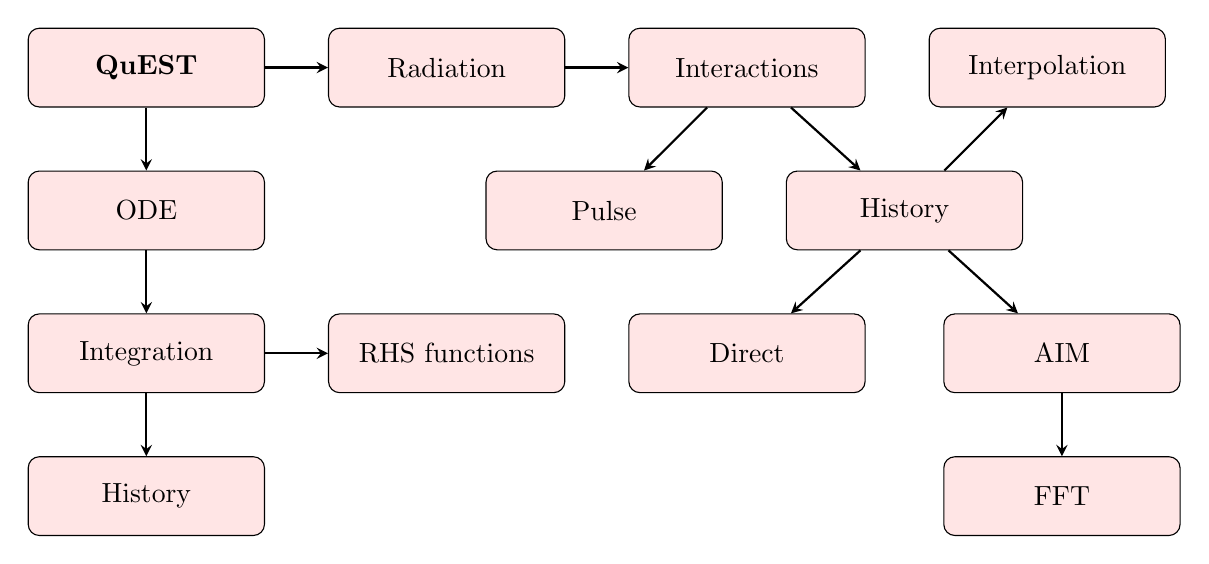
\begin{tikzpicture}[node distance=0.8cm, >=latex]
      \tikzstyle{startstop} = [rectangle, rounded corners, minimum width=3cm, minimum height=1cm,text centered, draw=black, fill=red!10]
      \tikzstyle{io} = [trapezium, trapezium left angle=70, trapezium right angle=110, minimum width=3cm, minimum height=1cm, text centered, draw=black, fill=blue!30]
      \tikzstyle{process} = [rectangle, minimum width=3cm, minimum height=1cm, text centered, draw=black, fill=orange!30]
      \tikzstyle{decision} = [diamond, minimum width=3cm, minimum height=1cm, text centered, draw=black, fill=green!30]
      \tikzstyle{arrow} = [thick,->,>=stealth]

      \node (quest) [startstop] {\textbf{QuEST}};
      \node (ode) [startstop, below= of quest] {ODE};
      \node (radiation) [startstop, right= of quest] {Radiation};

      \draw [arrow] (quest) -- (ode);
      \draw [arrow] (quest) -- (radiation);

      \node (interactions) [startstop, right= of radiation] {Interactions};
      \node (integration) [startstop, below= of ode] {Integration};
      \node (history) [startstop, below= of integration] {History};
      \node (rhs) [startstop, right= of integration] {RHS functions};

      \draw [arrow] (radiation) -- (interactions);
      \draw [arrow] (ode) -- (integration);
      \draw [arrow] (integration) -- (history);
      \draw [arrow] (integration) -- (rhs);

      \node (pulse) [startstop, below= of radiation, xshift=2cm] {Pulse};
      \node (historyI) [startstop, below= of interactions, xshift=2cm] {History};

      \draw [arrow](interactions) -- (pulse);
      \draw [arrow](interactions) -- (historyI);

      \node (interpolation) [startstop, right= of interactions] {Interpolation};
      \node (direct) [startstop, below= of historyI, xshift=-2cm] {Direct};
      \node (aim) [startstop, below= of historyI, xshift=2cm] {AIM};

      \node (fft) [startstop, below= of aim] {FFT};

      \draw [arrow] (historyI) -- (interpolation);
      \draw [arrow] (historyI) -- (direct);
      \draw [arrow] (historyI) -- (aim);
      \draw [arrow] (aim) -- (fft);

    \end{tikzpicture}
  %\end{center}
\end{frame}

\begin{frame}[standout]
  Questions?
\end{frame}

\appendix

\begin{frame}{Lightning review of (linear) Green's functions}
  To solve the following differential equation for $a(x)$ \ldots
  \begin{equation*}
    \hat{\mathcal{L}}\qty[a(x)] = b(x)
  \end{equation*}
  \ldots it's far easier to \emph{first} find the Green's function,
  \begin{equation*}
    \hat{\mathcal{L}}\qty[g(x, x')] = \delta(x - x').
  \end{equation*}
  Then,
  \begin{align*}
    \hat{\mathcal{L}}\qty[a(x)] &= \int \delta(x - x') b(x') \dd{x'} \\
                                &= \int \hat{\mathcal{L}}\qty[g(x, x')] b(x') \dd{x'} \\
                   \Aboxed{a(x) &= \int g(x, x') b(x') \dd{x'}}
  \end{align*}
\end{frame}

\begin{frame}
  \begin{block}{Laplace equation}
    \begin{equation*}
      \laplacian g(\vb{r}, \vb{r}') = -4 \pi \delta(\vb{r} - \vb{r}') \implies g(\vb{r}, \vb{r}') = \frac{1}{\abs{\vb{r} - \vb{r}'}}
    \end{equation*}
  \end{block}

  \begin{block}{Wave equation}
    \begin{equation*}
      \qty(\laplacian - \frac{1}{c^2}\pdv[2]{t}) g^{(4)} = -4 \pi \delta^{(4)} \implies g(\vb{r}, t; \vb{r}', t') = \frac{\delta(\vb{r} - \vb{r}')}{\abs{\vb{r} - \vb{r}'}} \delta\qty(t - t' - \frac{\abs{\vb{r} - \vb{r}'}}{c})
    \end{equation*}
  \end{block}
\end{frame}

\begin{frame}
  \begin{columns}[T]
    \column{0.5\textwidth}
      \centering
      \begin{tikzpicture}[
  declare function = {
    basis(\x) = 
      and(-1 <= \x, \x < 0)*(1+x)*(2+x)*(3+x)/6 +
      and(0  <= \x, \x < 1)*(1-x)*(1+x)*(2+x)/2 +
      and(1  <= \x, \x < 2)*(1-x)*(2-x)*(1+x)/2 + 
      and(2  <= \x, \x < 3)*(1-x)*(2-x)*(3-x)/6 + 
      or(\x <-1, \x > 3)*0;
  }
  ]

  \begin{axis}[
      %xtick={-4, -3, -2, -1},
      minor x tick num={4},
      minor y tick num={4},
      legend style={fill=none},
      width=\textwidth,
      height=0.6\textheight
      %xticklabels={$-4\Delta t$, $-3\Delta t$, $-2\Delta t$, $-\Delta t$}
  ]
  
  \addplot[very thick, domain=-1:3, smooth, samples=256] {basis(x)};
  \legend{$T(t/\Delta t)$}
  \end{axis}
\end{tikzpicture}


    \column{0.5\textwidth}
      \begin{block}{Space/time discretization}
        \begin{equation*}
          \tilde{\vb{P}}(\vb{r}, t) = \sum_{\ell = 0}^{N_s - 1} \sum_{m = 0}^{N_t - 1} \tilde{\mathcal{A}}_\ell^{(m)}\vb{S}_\ell(\vb{r}) T(t - m \, \Delta t)
        \end{equation*}
      \end{block}
      \begin{itemize}
        \item $\vb{S}_\ell(\vb{r}) = \vb{d}_\ell \delta(\vb{r} - \vb{r}_\ell)$
        \item $T(t) \rightarrow$ Lagrange polynomials
          \begin{itemize}
            \item causal, interpolatory, differentiable
          \end{itemize}
      \end{itemize}
  \end{columns}
\end{frame}

\end{document}
